\documentclass[a4paper,11pt,twocolumn]{article}
\usepackage[utf8]{inputenc}
%\usepackage[italian]{babel}
\usepackage{comment}
%\usepackage{lipsum}
\usepackage{float}
\usepackage{graphicx}
\usepackage[font=small,labelfont=bf]{caption}
\usepackage{multirow}
\usepackage{hyphenat}
\usepackage{sectsty}
%\usepackage{subfigure}
%\usepackage{color}
%\usepackage[dvipsnames]{xcolor}
%\sectionfont{\bfseries\Large\raggedright}

%\usepackage{hyperref}

%\hypersetup{hidelinks}

\allsectionsfont{\raggedright}
\graphicspath{ {images/} }

\usepackage{listings}
\usepackage{color}
\usepackage[svgnames]{xcolor}
\definecolor{dkgreen}{rgb}{0,0.6,0}
\definecolor{gray}{rgb}{0.5,0.5,0.5}
\definecolor{mauve}{rgb}{0.58,0,0.82}

\lstset{frame=tb,
  language=python,
 aboveskip=3mm,
  belowskip=3mm,
  showstringspaces=false,
  columns=flexible,
  basicstyle={\small\ttfamily},
  numbers=none,
  numberstyle=\tiny\color{gray},
  keywordstyle=\color{blue},
  commentstyle=\color{dkgreen},
  stringstyle=\color{mauve},
  breaklines=true,
  breakatwhitespace=true,
  tabsize=3
}

%\bibliographystyle{apalike}
\usepackage[dashed=false, maxnames=1, uniquelist=false, backend=bibtex,sorting=none,style=authoryear-icomp]{biblatex}
\renewbibmacro{in:}{}
\setlength{\bibhang}{0pt}
\renewcommand*{\bibfont}{\small}
\renewcommand*{\finentrypunct}{}
\addbibresource{bibliography.bib}


%\usepackage[T1]{fontenc}
\usepackage[hyperfootnotes=false]{hyperref}

\pagestyle{headings}


\title{Detection of a transiting Hot Jupiter around WASP-44}
\author{Adriana Barbieri \and Alessandro Bianchetti}

\begin{document}
\maketitle

\begin{abstract}

\emph{In the following report we work on WASP-44 b, an exoplanet orbiting 
around its G-type parent star, located in the constellation of Cetus. 
We first examine its atmospheric parameters and derive its mass and 
radius (\cite{Morton}). Then, we correct for limb darkening effect through different methods 
(\cite{claret2011}, \cite{claret2017}, \cite{claret2018}). We also take 
some images obtained with Copernico telescope at the Asiago Observatory into consideration 
and, after proper correction, we use them to extract the light curve of 
the alleged planet.}

\end{abstract}

\section{Introduction}

Confirmed exoplanets are growing in number year by year, and transit method 
is nowadays a widespread and hugely successfull detection method. Most planets indeed are by now discovered 
by tracing the lightcurve and searching for any sign of a weakening in the 
flux.
\begin{figure}[H]
    \centering  
    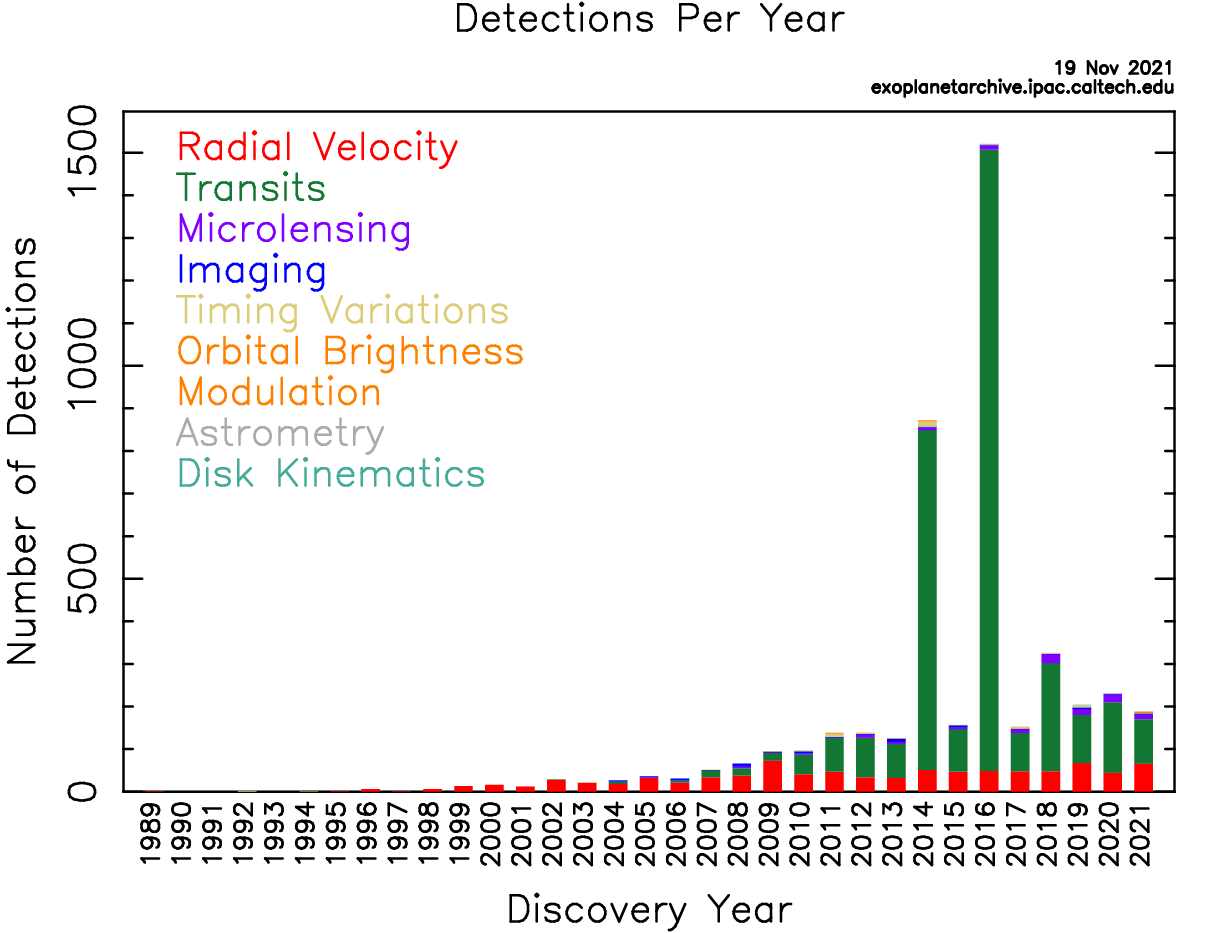
\includegraphics[scale=0.15, angle=0]{../pictures/exo_dischist.png}
    \caption{Confirmed exoplanets distribution per year of detection via different methods. Credits to \textit{https://exoplanetarchive.ipac.caltech.edu/}}
\end{figure}
In this report we focus on WASP-44 b, a Jupiter-size planet orbiting around 
a G-type star, located in the constellation of Cetus.
Among the numerous available reports on the planet, we decided to make a 
conservative choice and avoid any result which is not inferred via 
spectroscopy. This leads us to rule out several papers regarding our target of interest and exclusively
 work with the discovery paper (\cite{Anderson}). In this paper, estimates 
of the atmospheric parameters of WASP-44 are provided via an analysis of 
the width of the spectral lines.

%\section{Instruments}




\section{The transit method }

The transit method is a photometric indirect method of detection of exoplanets, which consists in the observation of a drop in the flux of a star due to the transit of a planet across the stellar disk. 

The subsequent variation of the measured stellar luminosity is proportional to the ratio of the projected areas of the planet and the star, or equivalently, the dimming of the flux is proportional to the ratio of the square of the respective radii; therefore, known the radius of the star from its spectrum, the radius of the planet can be easily obtained from the measured depth of the flux.

Moreover, if combined with radial velocities measurements, this method allows to compute also the average densitiy of the exoplanet.

It is important however to notice that limb darkening, stellar activity and atmospheric effects may pollute the observational transit curve and must be all taken into account.

The modelled transit light curve is distinguished by a characteristic trapezoidal shape, whose main geometrical parameters are the impact parameter, the ingress/egress and transit duration, and the transit depth.
\begin{figure}[H]
    \centering  
    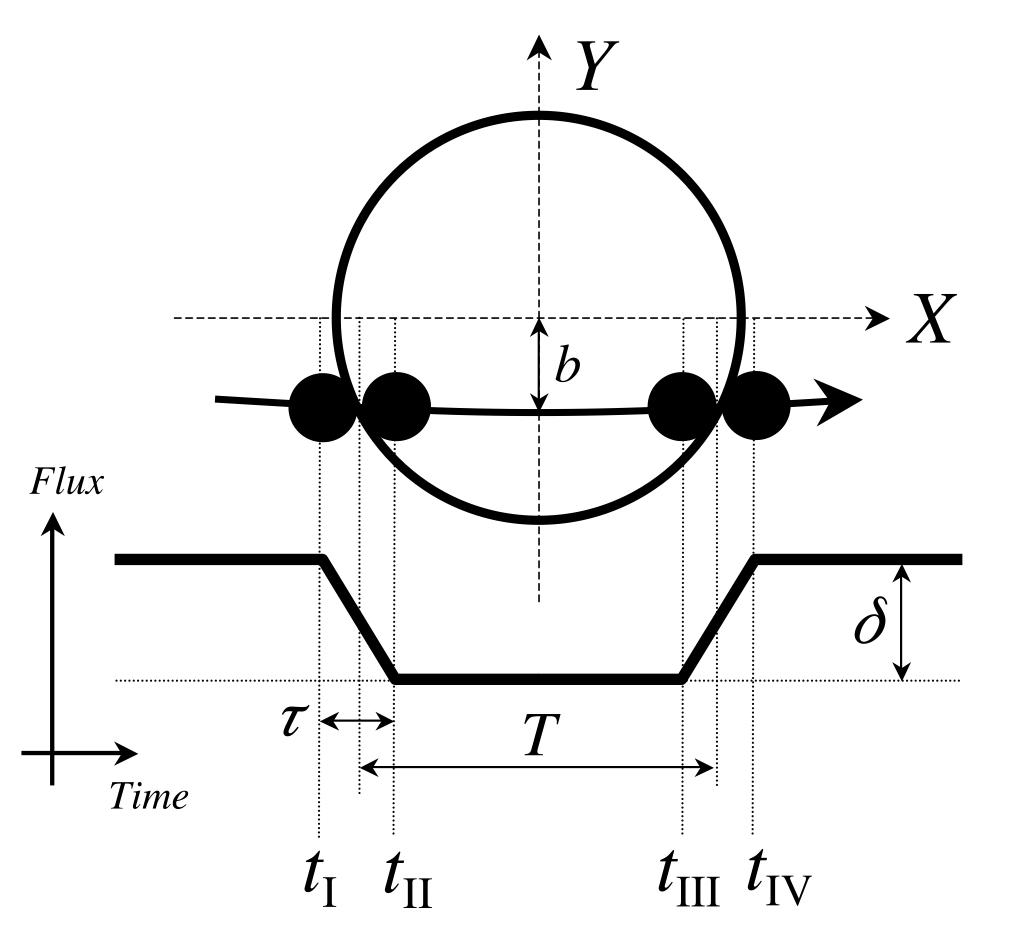
\includegraphics[scale=0.18, angle=0]{../pictures/transit.jpeg}
    \caption{Simplified transit light curve. Credits to \textit{Winn [2010]}}
\end{figure}
The geometry of the system places a strong constraint on the inclination of the orbital plane of the planet with respect to the line of sight: the transit can be observed exclusively for almost edge-on orbits, meaning orbital planes that are as parallel as possible to the line of sight. This condition yealds a low probability of detection, which in turn requires a huge number of target stars to carry on successfull observations.

Furthermore, at least two transits are required to determine the orbital period of the extrasolar planet candidate, and since the duration of the transit is very short compared to the orbital period, continuous and prolonged observations are required in order to detect it.

It is of capital importance to be aware of the selection biases that are intrinsic to this method (and to the current available technology): indeed it yealds the largest detection probability for large massive planets orbiting very close to small and quiet stars, thus selecting Hot Jupiters around late type stars as ideal targets.

\section{Preliminary steps}

\subsection{Inferring mass and radius}

The $H_{\alpha}$ line was used to determine the effective temperature (Teff ),
while the $NaI$ D and $MgI$ b lines were used as surface gravity
($\log{g^*}$) diagnostics (\cite{Anderson}). The elemental abundances, including $[Fe/H]$ 
were determined from equivalent width measurements of several clean and 
unblended lines. This led to proper estimation of the atmospheric parameter 
triplet $T_{eff}$, $\log{g^*}$ and $[Fe/H]$. Quoted errors include statistical 
uncertainties only. In the same conservative spirit we 
previously showed, we add in quadrature a further term to the errors of 
all three parameters (\cite{Sousa}). We are in fact more interested in an 
accurate result rather than in a precise one.
This leads to the following results 
\begin{center}
    \begin{tabular}{ccc}
    \hline
    $T_{eff}$ (K) & $\log{g^*}$ & $[Fe/H]$ \\
    \hline
    $5400 \pm 162$ & $4.5 \pm 0.2$ & $0.06 \pm 0.11$ \\
    \hline
    \end{tabular}
\end{center}
We then ran \textit{isochrones} (\cite{Morton}), with Bayesian approach, 
with posterior sampling performed by \textit{MultiNest} and including Gaia 
parallax $p=2.764 \pm 0.020$ $\mu as$. These are the results of the 
analysis:
\begin{center}
    \begin{tabular}{cc}
    \hline
    Parameter & Value \\
    \hline
     $M (M_{\odot})$ &  $0.95\pm0.05$ \\
     $R (R_{\odot})$ & $0.93 \pm 0.01$  \\
     $\rho (\rho_{\odot})$ & $1.19 \pm 0.09$ \\
     $age (Gyr)$  & $4.8^{+3.5}_{-2.9}$ \\
    \hline
    \end{tabular}
\end{center}
Huge errors on the age estimate are pretty common for this analysis, since 
stars with this mass evolve very slowly along the Main Sequence.

%Mass (Msun)     :     0.952972      0.954230     -0.050431     0.047930
%Radius (Rsun)   :     0.928634      0.928171     -0.011579     0.012578
%Density (ro_sun):     1.192031      1.194963     -0.093708     0.088772
%age (Gyr)       :     4.836685      4.533456     -2.908078     3.512064

\subsection{Limb darkening correction}

Limb darkening is an important effect that cannot be neglected when observing a star.
In short, the edges of the luminosity profile 
of a star always look darker than the core: this occurs because there is a physical, constant 
distance $L$ at which the optical depth is equal to unity, further than which 
the observations are not possible since photons are completely absorbed and do not reach the observer. This characteristic size, 
however, can extend deep inside the hot layers of the star if we look straight 
to the center, being $L$ radial, while it can stop at the colder, outer layers 
if we look at the edges of the star, since $L$ and our line of sight (LoS) are not radial 
anymore.
\begin{figure}[H]
    \centering  
    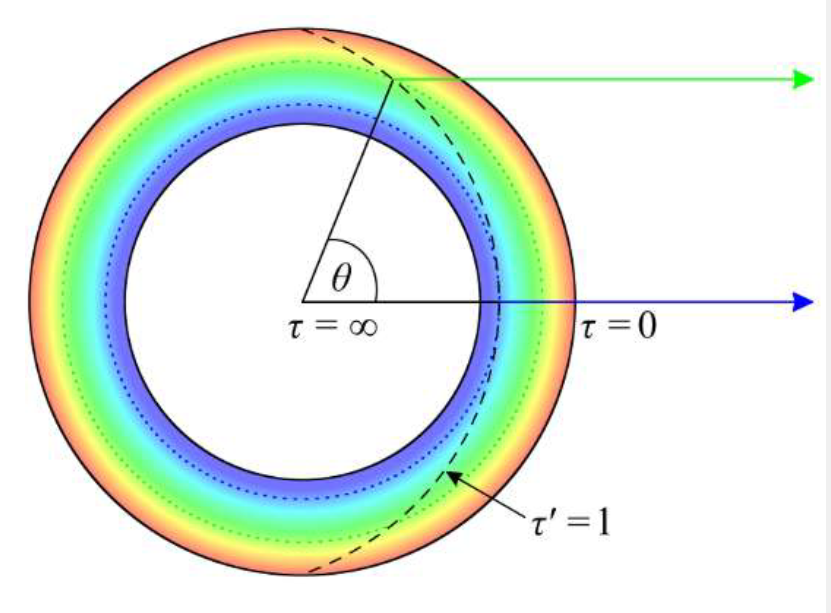
\includegraphics[scale=0.25, angle=0]{../pictures/limb_darkening.png}
    \caption{Limb darkening effect scheme. Credits to \textit{https://ediss.sub.uni-hamburg.de}}
\end{figure}
Correcting for this effect may be challenging. Indeed we can measure it 
directly only for the Sun, while we need to model it somehow for any other 
star, thus figuring out a proper law for the intensity decrease $I(\mu)$, 
where $\mu = \sqrt{1-r^2}$. Many choices are plausible at this point: a 
uniform behaviour, a linear, a quadratic, a square-root or a 
logarithmic law are all valid guesses. Parametrizing such laws introduces 
the so-called \textit{LD-coefficients}, which will depend on the stellar 
parameters. Knowing the latter relationship (for instance calibrating it 
based on a large sample of stars) allows to obtain the coefficients directly 
from the atmopsheric parameters. 
The alternative way is fitting the light curve leaving the coefficients as free parameters.

The choice of the functional dependence on $\mu$ is a delicate one. Multiple 
approaches can be followed, basing on different papers. This analysis is 
addressed in \ref{sect:app_A}.


\section{TASTE data analysis}

Before actually analysing data from TASTE, we need to properly correct them.
Then, we're going to have a look at and correctly format them, preparing 
the configurations file for the PyORBIT run. 


\subsection{Bias and flat field correction}
CCD s(Charged Coupled Devices) are the privileged detectors for photon counting, 
due to their high quantum efficiency. The images produced are \textit{raw}
and must be properly \textit{pre-reduced} before being analysed. Pre-reduction 
goes through different steps:
\begin{itemize}
    \item \textbf{bias} is the
    individual pixel-to-pixel offset level, and it is a zero-exposure instrumental 
    factor, thus it is always an added contribution to any signal. Therefore it must 
    be removed in order to isolate the photons of astrophysical origin. The root mean square 
    of the bias corresponds to the so-called \textit{readout noise}. We perform an 
    average across all the pixels to get an estimate of the bias;
    \item a \textbf{flat field} is a calibration image obtained by illuminating
    homogeneously the pupil of the telescope, using twilight sky or appropriate, 
    back-lighted screens. This correction factor is to be applied on each pixel and 
    then also normalised, after the overall bias correction;
    \item \textbf{differential photometry} is a great way to keep track of any noise
    variation. The idea is to take a reference star close enoguh to the target: any 
    environmental or instrumental variation will affect both sources. Working with 
    flux ratios will make only astrophysical variations evident!
\end{itemize}
For pre-reductions steps, we use the code \textit{huggy}. We first perform bias
correction, than the flat field correction. The corrected images are ready for 
aperture synthesis.

\subsubsection{Bias correction}
We run \textit{huggy-bias.e} inputting the raw images. 
\begin{lstlisting}
huggy-bias.e A*.fits
\end{lstlisting}
Many bias images are produced,
displaying the zero offset of the pixel board. \textit{Master bias} is the average 
of all these files. Plotting the intensities of the offset level of the pixels yields 
a concrete view of the correction.
\begin{figure}[H]
    \centering  
    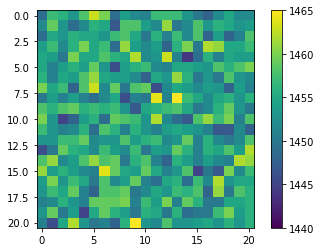
\includegraphics[scale=0.32, angle=0]{../pictures/pre-reduction/bias.png}
    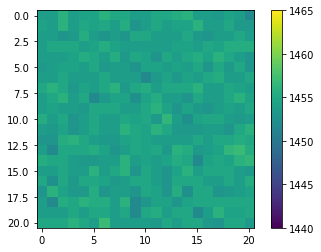
\includegraphics[scale=0.32, angle=0]{../pictures/pre-reduction/master_bias.png}
    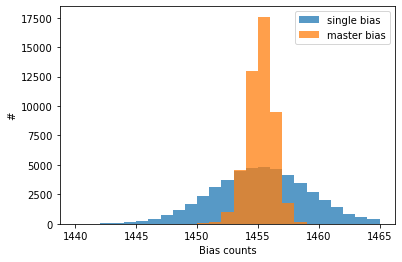
\includegraphics[scale=0.35, angle=0]{../pictures/pre-reduction/bias_comp.png}
    \caption{Comparison between random bias frame and master bias}
\end{figure}
Note that the master bias frame distribution is peaked and much closer to a 
unique constant value, as all pixels behaved in the same way, like in an 
ideal situation. We can see this even numerically, by looking at the 
dispersions of the above distributions: $\sigma_{rb} = 3.82$ and 
$\sigma_{mb} = 0.89$.

\subsubsection{Flat field correction}
We now run \textit{huggy-flat.e} inputting a normalization fraction, 
meaning the fraction of pixels we want to account for, ruling out the 
sides which are often polluted by overscan columns. These are visible 
in the form of dark stripes on the sides of any flat field take. Then 
we have to input the overscan values, usually set to 0. Subsequently,
we need to provide the master bias file, which will be subtracted from 
the data. Finally, we input all the available flat fields.
\begin{lstlisting}
huggy-flat.e 0.9 0 0 mb.fits A*.fits
\end{lstlisting}
This will produce an outpute file showing the average response of
pixels to an external light source. Minor differences in such response 
are important and must be accounted for.
\begin{figure}[H]
    \centering  
    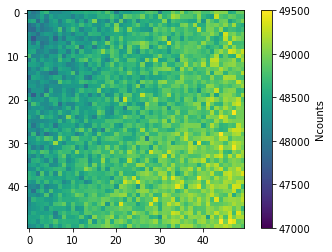
\includegraphics[scale=0.32, angle=0]{../pictures/pre-reduction/flat.png}
    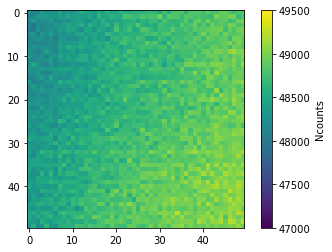
\includegraphics[scale=0.32, angle=0]{../pictures/pre-reduction/master_flat.png}
    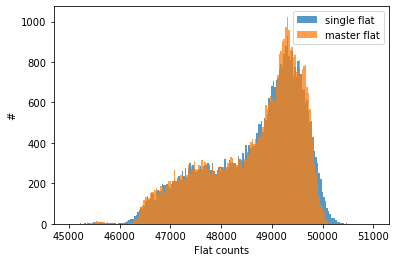
\includegraphics[scale=0.35, angle=0]{../pictures/pre-reduction/flat_comp.png}
    \caption{Comparison between random flat field and master flat}
\end{figure}

\subsection{Final correction}
The final step is applying the correction files obtained in the 
previous parts.
\begin{lstlisting}
huggy-correct.e mb.fits mfn.fits A*.fits
\end{lstlisting}
The final correction code requires the master bias and the normalised 
master flat, and of course all the target images, that are all going to be 
 corrected.



\subsection{Extracting the light curve}
We are approaching the very heart of this analysis, preparing for 
aperture synthesis. We now need to display the science images, make 
sure to identify the correct target and select a proper background 
analysis around it. To do that, we have to properly circle the source 
and create a slightly larger circle around it (we used the the $ds9$ tools).
The same procedure must be repeated (with the same inner and outer radii) 
on a properly selected reference star, close to and roughly as bright 
as the target. We hereby report the coordinates of the target and of the 
chosen reference star, in pixel units.
\begin{center}
    \begin{tabular}{ccc}
    \hline
     & $x_c$ & $y_c$ \\
    \hline
    Target    &  170  &  37    \\
    Reference & 288 & 57  \\
    \hline
    \end{tabular}

    \medskip

    $R_{in} = 11$, $R_{out} = 20$
\end{center}
Now we need to call \textit{huggy-psf.e} and input the coordinates of the 
center of the target, the inner and outer radii, and a random corrected 
image.
\begin{lstlisting}
huggy-psf.e x0 y0 Rin Rout A*.fits
\end{lstlisting}
This yields information about the Point Spread Function, meaning how the 
the flux is distributed as a function of the distance from the core of 
the source. The ouput displays the radii at which we find 90, 95 and 99\%
of the total flux. The three apertures in pixel units are $a_0=4.71$, 
$a_1=5.97$ and $a_2=8.76$, respectively for 90, 95 and 99\%. 
We take note of this output. 

%    re-estimated x (pix):  169.85
%    re-estimated y (pix):   37.69

Photometry analysis is carried out by \textit{sentinel.e}, which needs 
the coordinates of the target and of the reference stars, followed by 
the radii of two selected apertures from the previous output. Also, we need 
again inner and outer radii of the selected region for the analysis, as well 
as the full-corrected images of the target. 
\begin{lstlisting}
sentinel.e x0 y0 xr yr a1 a2 Rin Rout c A*.corr.fits
\end{lstlisting}
where $c=\{1,2\}$ selects the centroiding method (gaussian/moment). For a star
fainter than average like ours ($J\approx 11$) the recommended choices for 
the apertures are 90 and 95\%, in order to make sure not to run into 
saturation. However, all three possibilities were tested. 

%our choices are $a_1=4.71$ and 
%$a_2=5.97$, corresponding to 90 and 95\%. 

\medskip

The \textit{sentinel} output is the starting point for TASTE analysis. This file 
contains the main information about the target and the sky, keeping track of the 
respective photometries. In fact, we check the evolution of the 
sky background throughout the observation session, and also to the behaviour 
of the reference star (\ref{fig:sky-ref}).
\begin{figure}
    \centering  
    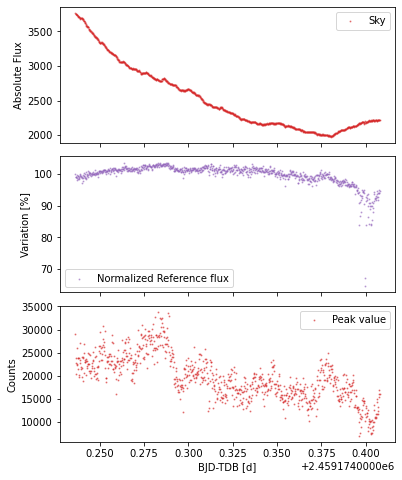
\includegraphics[scale=0.5, angle=0]{../pictures/taste/sky-ref.png}
    \caption{Upper panel: sky background flux, every point is the median of the anulus
    formed by $R_{in}$ and $R_{out}$. Middle panel: reference star flux, 
    normalised to the first measurement. Bottom panel: peak points of the 
    flux inside the defined aperture.}
    \label{fig:sky-ref}
\end{figure}
The sky flux has been constantly decreasing in time, so we expect less and less 
disturbance as the observation proceeds. The reference star, on the other hand 
seems to be pretty stable in terms of flux. 
We also want to make sure that reference star are correctly comoving: to do that, 
we plot the variation in position at every time step and make sure we have 
similar motion (\ref{fig:target-ref_position}). Plotting FWHM reveals an increasing trend, at odds with 
the sky pattern.
\begin{figure}
    \centering  
    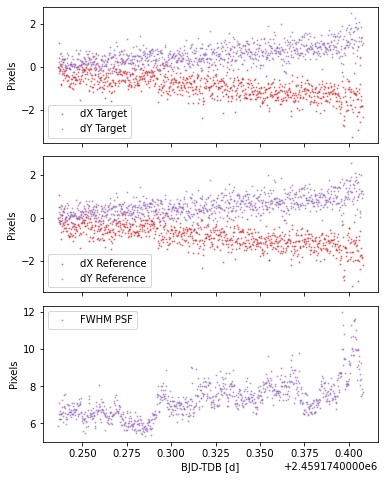
\includegraphics[scale=0.5, angle=0]{../pictures/taste/target-ref_position.png}
    \caption{Upper and middle panel: target and reference star show the same 
    coordinate variation in the CCD. Bottom panel: full width half maximum 
    of the peak flux.}
    \label{fig:target-ref_position}
\end{figure}
Next, we compare the flux plot of all three different aperture we have 
chosen (\ref{fig:apertures}).
\begin{figure}
    \centering  
    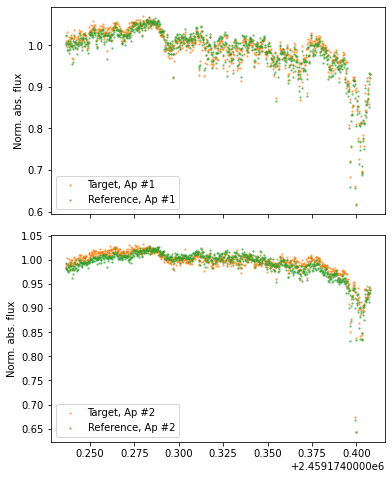
\includegraphics[scale=0.5, angle=0]{../pictures/taste/apertures.png}
    \caption{From top to bottom: 90, 95 and 99\% apertures, showing 
    both the target and reference star. Dispersion is reduced as the 
    aperture grows.}
    \label{fig:apertures}
\end{figure}
The second case (99\%) seems to be slighly less noisy: that's our first clue 
that this aperture might be the best suited choice for the aperture analysis.
As a further goodness check, one may take a look at the peak value trend of 
the target source and compare it to the saturation level. We also plot the 
reference star flux to see whether they are above the quality threshold.
\begin{figure}
    \centering  
    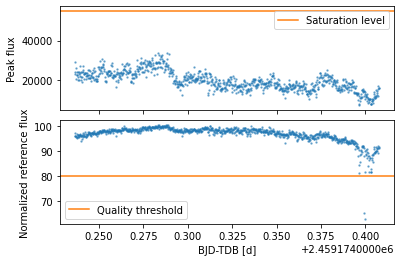
\includegraphics[scale=0.5, angle=0]{../pictures/taste/saturation-quality.png}
    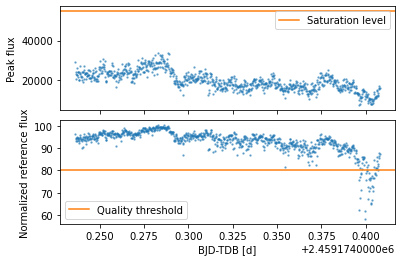
\includegraphics[scale=0.5, angle=0]{../pictures/taste/saturation-quality2.png}
    \caption{Upper panel: narrow apertures, bottom panel: wider apertures.
    In both cases the peak value is well below the saturation limit, and 
    we also see that the reference data are above the required threshold. 
    A few points at late times are below the quality factor for the 90-95\% 
    case, thus supporting the choice of the widest aperture at 99\%.}
    \label{fig:saturation-quality}
\end{figure}

We can can finally visualise the transit in all three cases. To do that, we 
plot the ratio between target and reference star: \textit{differential 
photometry} helps us get rid of systematic errors affecting both sources.
We still see that the wider aperture seems to have less dispersion than 
the other case, and we keep that in mind.
\begin{figure}
    \centering
    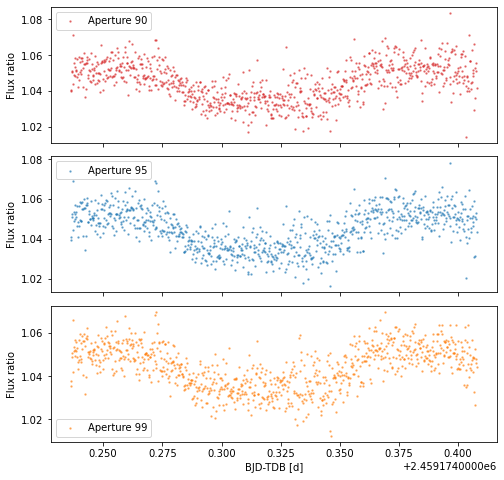
\includegraphics[scale=0.5, angle=0]{../pictures/taste/transits.png}
    \caption{Transit image for growing aperture, top to bottom. Note that 
    the above case (90\%) shows the most outliers.}
    \label{fig:transits}
\end{figure}


In order to evaluate the depth of the transit, we need to identify the "height" 
of the continuous level: to do that, we need to exclude the transit datapoints 
and try out a polynomial fit, hoping to find a perfectly horizontal line. That 
will be our reference trend for the stellar flux.
\begin{figure}
    \centering  
    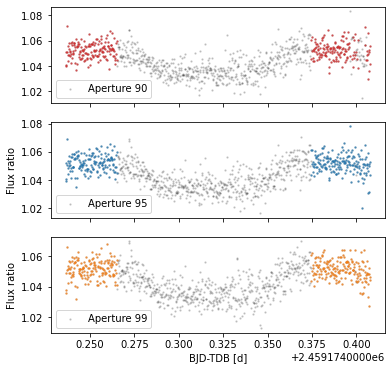
\includegraphics[scale=0.5, angle=0]{../pictures/taste/fit_setting.png}
    \caption{Time boundaries for the transit are roughly ballparked to 
    prepare a proper, flat dataset to fit with a straight line.}
    \label{fig:fit_setting}
\end{figure}
To perform the fit, we ruled out all the points during the transit by roughly 
selecting an ingress and egress time. A quadratic law ($p_0 x^2 + p_1 x +p_2$)
was chosen to set things up in the most general case. A least square fitting 
via numpy function \textit{np.polyfit} yields Fig.\ref{fig:fit}.
\begin{figure}
    \centering  
    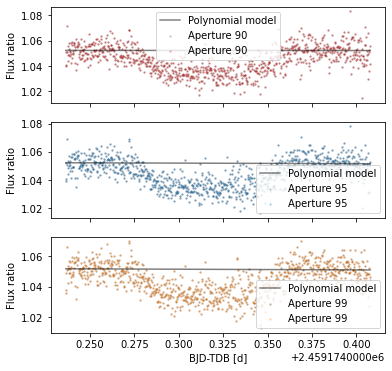
\includegraphics[scale=0.45, angle=0]{../pictures/taste/fit.png}
    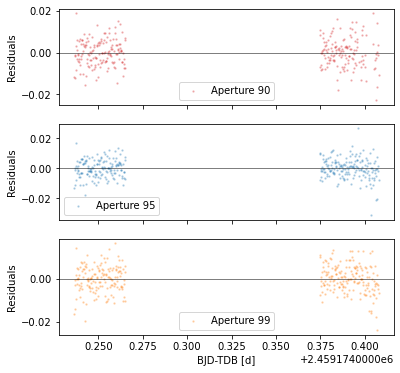
\includegraphics[scale=0.45, angle=0]{../pictures/taste/residuals.png}
    \caption{Horizontal fit and residuals for the three cases.}
    \label{fig:fit}
\end{figure}
\begin{center}
    \begin{tabular}{cccc}
    \hline
    \# ap & $p_0 (\cdot 10^{-10})$ & $p_1 (\cdot 10^{-7})$ & $p_2 ( \cdot 10^3)$ \\
    \hline
    90 & $-1.19$ & $1.43$  & $0.72$\\
    95 & $-7.98$ & $1.43$  &  $4.82$\\
    99 & $-8.98$ & $1.42$  & $5.43$\\
    \hline
    \end{tabular}
\end{center}
We immediately notice that both $p_0$ and $p_1$ are well compatible with zero,
meaning that only a constant term survives: that represents the level of the 
continuous. 

After the fit, we also considered discarding outliers: however, a quick 
analyisis reveal that all point are well within $5\sigma$. Actually, 
except for the 90\% aperture, even a more strict $3\sigma$ criterion 
would not rule out any data point.

We display the standard deviation of the points of the 
continuous with respect to the linear fit. These quantify scattering and 
indicate that the 99\% aperture is indeed the best photometric choice, 
having the smallest standard deviation.
\begin{center}
    \begin{tabular}{cc}
    \hline
    $\sigma_{90}$ & $0.0063$ \\
    $\sigma_{95}$ & $0.0061$ \\
    $\sigma_{99}$ & $0.0059$ \\
    \hline
    \end{tabular}
\end{center}





\section{TESS data analysis}


%Conversion from fit parameters to physical parameters

\subsection{Light curve extraction via aperture photometry}

WASP-44 was observed by TESS (Transiting Exoplanet Survey Satellite) in 120 s cadence mode during observations of sector 3, between 2018 September 20 and October 17.

The photometric observations for WASP-44 were reduced by the Science Processing Operations Center (SPOC) pipeline (\cite{Jenkins}).

From ExoFOP-TESS \footnote{Exoplanet Follow-up Observing Program for TESS website, to be found at https://exofop.ipac.caltech.edu/tess/} 
we retrieved the TIC (TESS Input Catalog) identification number for our target star, 12862099.
We were able then to download the 2-min cadence target pixel file (TPF), the SAP (Simple Aperture Photometry) and 
PDCSAP (Pre-search Data Conditioning Simple Aperture Photometry) flux files from the Mikulski Archive for Space 
Telescopes (MAST)\footnote{https://mast.stsci.edu/portal/Mashup/ Clients/Mast/Portal.html}, after a previous selection 
of the data exclusive to the TESS mission.



We performed a preliminary contamination check with \textit{tpfplotter} \footnote{https://github.com/jlillo/tpfplotter.git}, 
aiming to establish whether our default photometric aperture includes any contaminant star that may cause a dilution of the transit.

By running
\begin{lstlisting}
python tpfplotter.py 12862099 --maglim 6 --SAVEGAIA
\end{lstlisting}
we obtained the following tpf plot \ref{fig:tpfplot}, which shows how only one star is present within the mask, 
but since it is over 4 magnitudes fainter than the target in the G band, it does not constitutes a contaminant and can therefore be ignored.
\begin{figure}
    \centering
    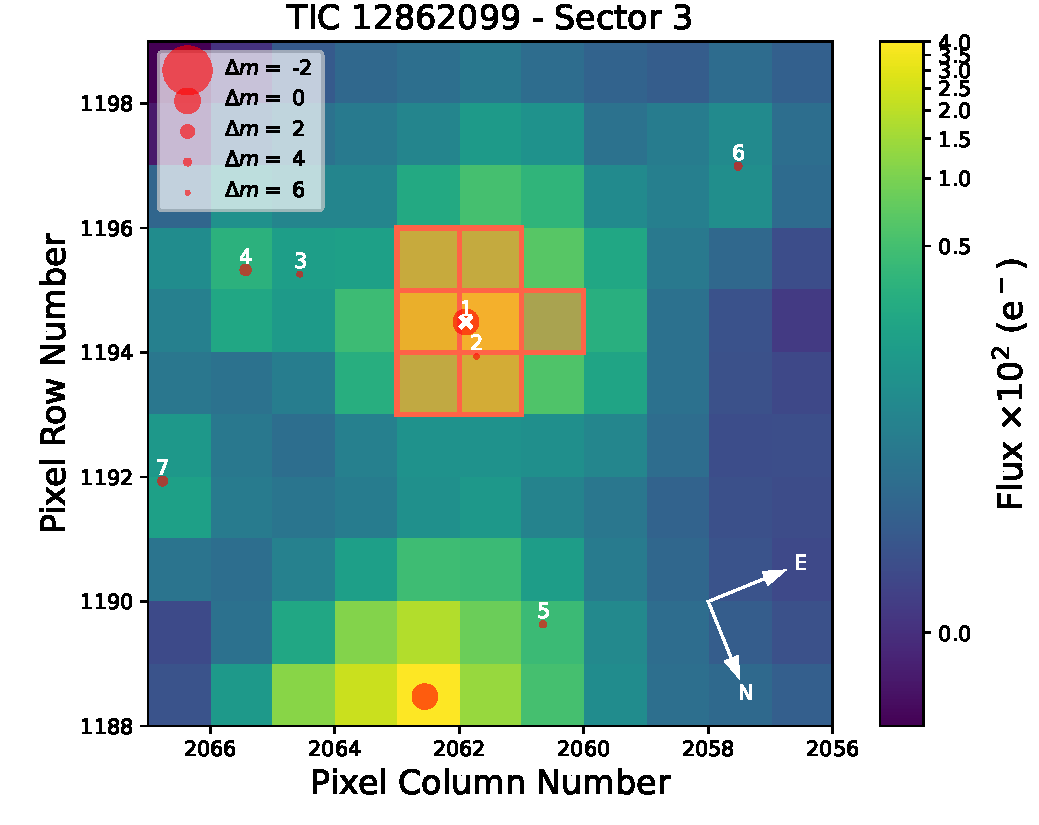
\includegraphics[scale=0.4, angle=0]{../pictures/tess/TPF.pdf}
    \caption{TPF plot.}
    \label{fig:tpfplot}
\end{figure}


In order to obtain an independent confirmation of the signals
detected in the TESS light curve, we performed an iterative transit
search on the detrended light curve using the Transit Least Squares method.
%(TLS) algorithm (Hippke & Heller 2019)



We proceeded to perform aperture and time series photometry on the TPF in order to select only the 
pixels belonging to the optimal aperture; from the obtained calibrated pixels, we derived 
the transit and the background flux light curves. Afterwards we removed from the time series 
dataset of the optimal aperture all the TESS cadences flagged as anomalous or encoded as NaN, 
as can be seen in \ref{fig:tess} .

\begin{figure}
    \centering
    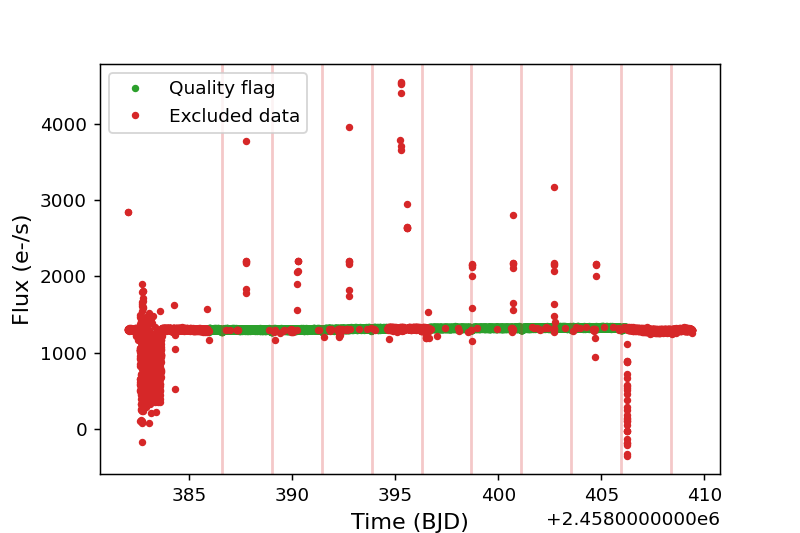
\includegraphics[scale=0.3, angle=0]{../pictures/tess/tess.png}
    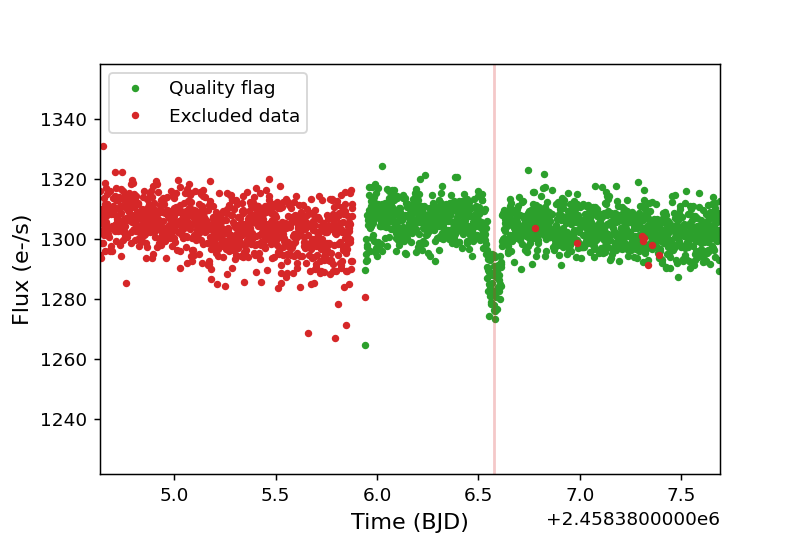
\includegraphics[scale=0.3, angle=0]{../pictures/tess/zoom.png}	
    \caption{Flux derived from the calibrated pixels (up) and detail of the first cadence (bottom).}
    \label{fig:tess}
\end{figure}



Subsequently we repeated the quality selection analysis on the lightcurve files (provided by the 
TESS team and obtained from the MAST portal as previously addressed), and plotted both the optimal 
aperture, the SAP and the PDCSAP fluxes thus obtained as a function of time. We can be sure of 
the correctness of the analysis we carried on from the observed overlapping between the optimal aperture and the SAP lightcurve. For our photometric analysis, however, we will make use of 
the PDCSAP light curve, being the PDCSAP flux usually cleaner than the SAP flux and corrected for systematic trends.


\begin{figure}
    \centering
    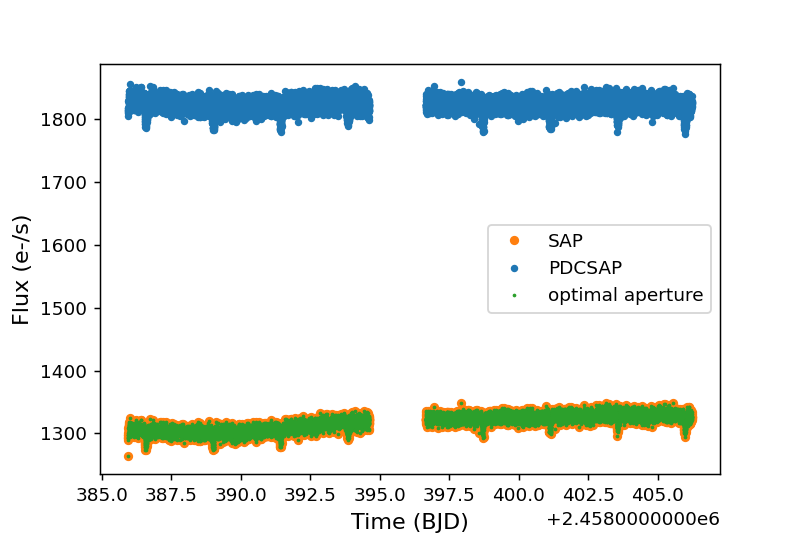
\includegraphics[scale=0.3, angle=0]{../pictures/tess/lightcurve.png}
    \caption{Optimal aperture, SAP and PDCSAP lightcurves.}
   %\label{fig:tess}
\end{figure}



\subsection{Detrending methods}

It is of capital importance to flatten and de-trend the light curve, meaning to correct for stellar activity, 
flares, gaps in the data and interrupted transits by removal of the curve modulation due to the stellar and instrumental systematics.
Via the \textit{WOTAN} package \footnote{https://github.com/hippke/wotan} (\cite{Hippke1}) we applied to the 
PDCSAP light curve a biweight filter with a time window of 1 d and a hspline filter with a time window of 2 d 
(\ref{fig:filters}); afterwards we normalized and folded the lightcurves, with the aim of studying the transits in phase (\ref{fig:Transits}).


\begin{figure}
   % \centering
    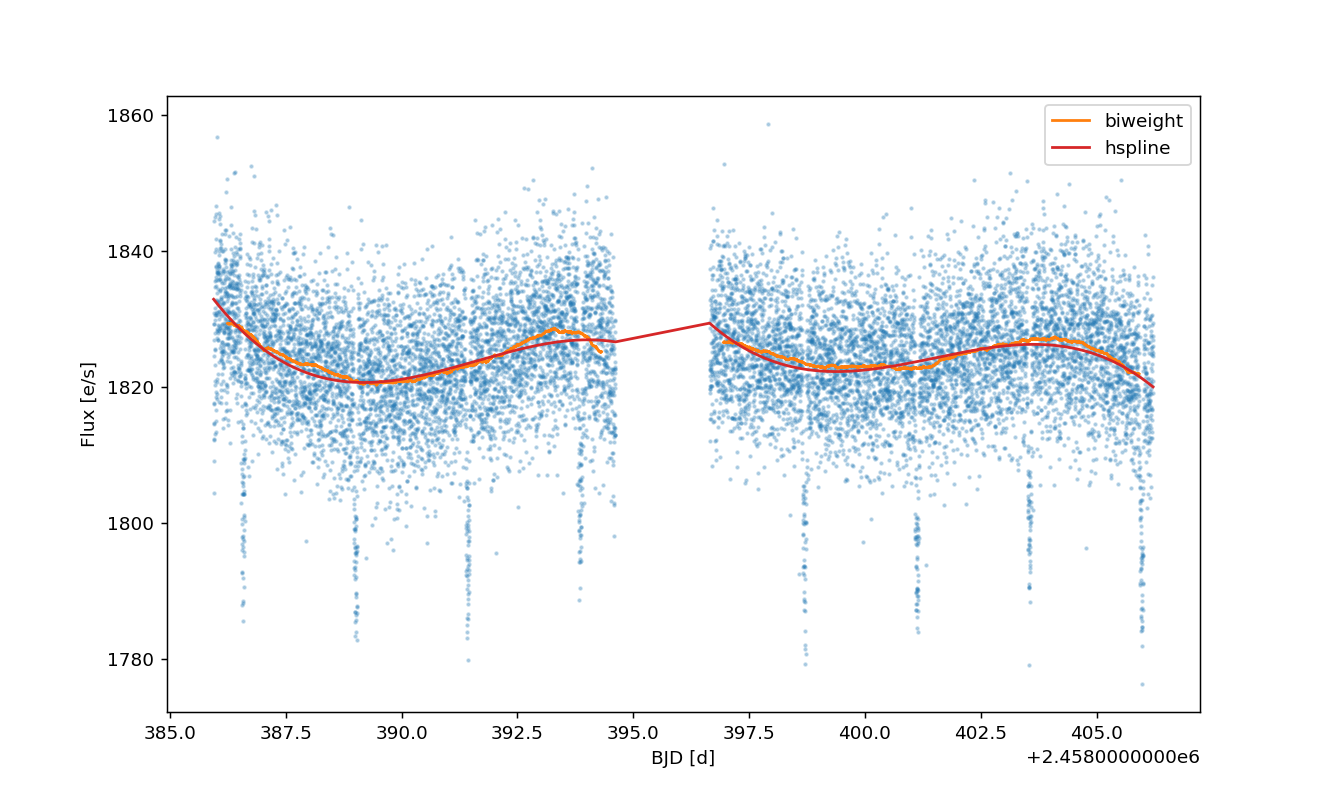
\includegraphics[scale=0.18, angle=0]{../pictures/tess/filters.png}
    \caption{Outliers exclusion and time windowing}
   \label{fig:filters}
\end{figure}



\begin{figure}
  %  \centering
    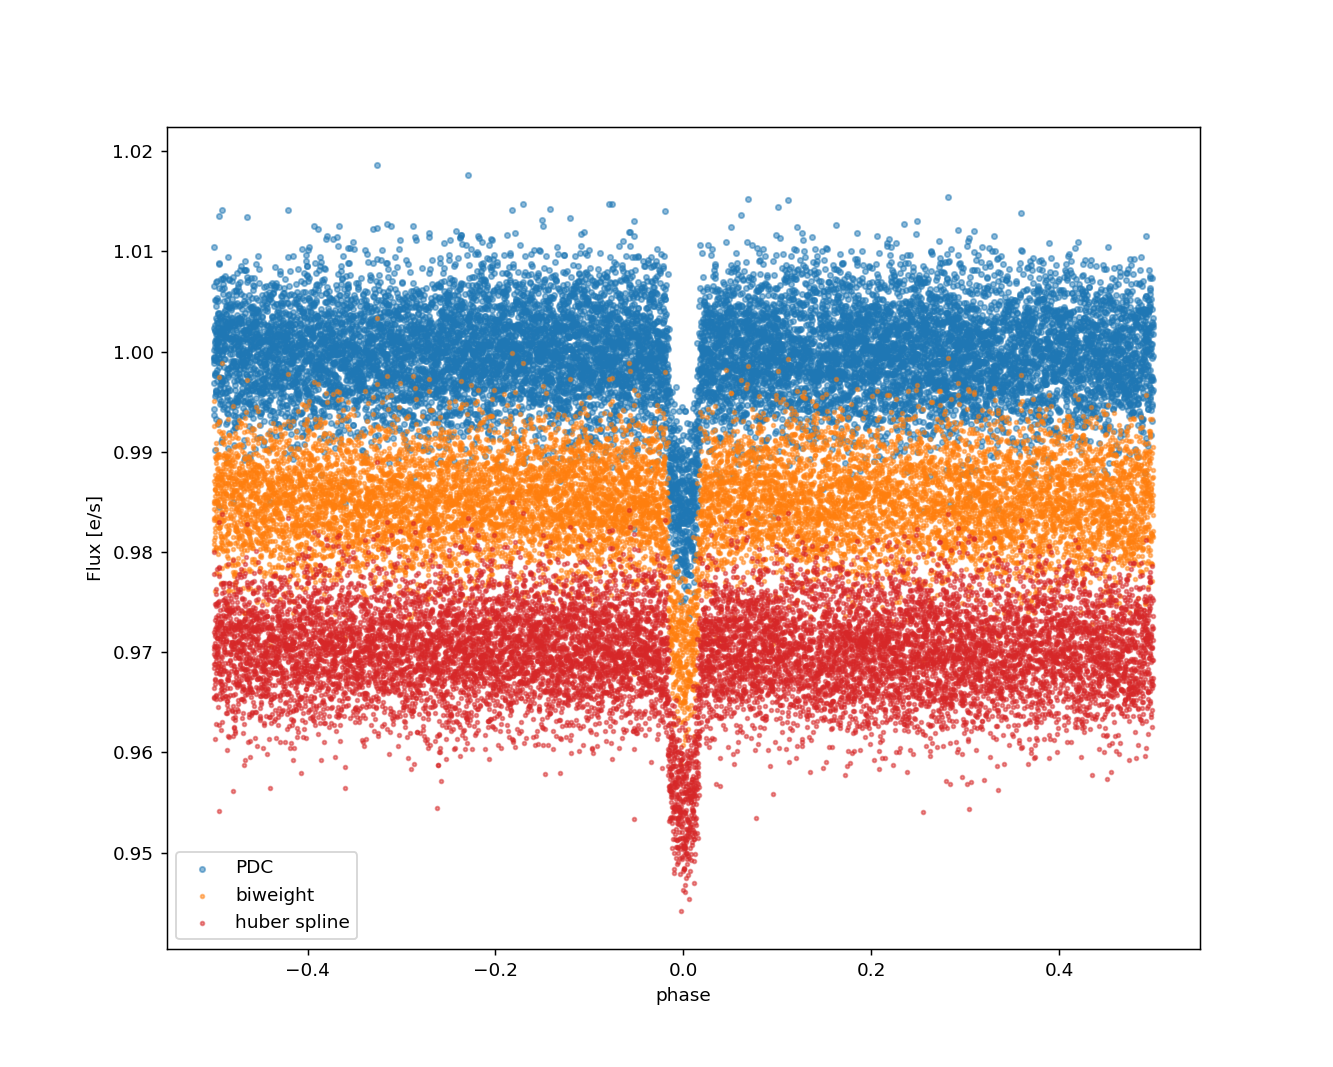
\includegraphics[scale=0.18, angle=0]{../pictures/tess/phase.png}
    \caption{Flattened and folded data}
   \label{fig:Transits}
\end{figure}


We obtained for the PDCSAP, biweight and hspline fluxes' standard deviations the values of 0.00440736, 0.00406469 and 
0.00407942 respectively. Therefore, having the smallest $\sigma$, we considered the flattened biweight lightcurve as the most accurate one.

\subsection{Identification of periodic signals}

We proceeded to perform an iterative  transit search on the detrended light curve in order to independently 
confirm the detection of the periodic signals in the TESS light curve.
We used  the Transit Least Squares (TLS) \footnote{https://github.com/hippke/tls} algorithm (\cite{Hippke2}), 
which offers one of the best method to detect planetary transits from time-series photometry.
Indeed it searches for transit-like features with stellar limb-darkening, includes the effects of planetary 
ingress and egress, analyses the entire data of the phase-folded light curve and yields a $\approx 10 \% $ higher 
detection efficiency (SDE) compared to the Box-fitting Least Square (BLS) method, therefore being more accurate but more time-consuming. 

We obtained the following periodgram and folded lightcurve with a SDE of 15.15413, a period of 2.42547 d, a central transit time of 
2458386.57308 BJD and a best transit duration of 0.07180 d.
 


\begin{figure}
   \centering
    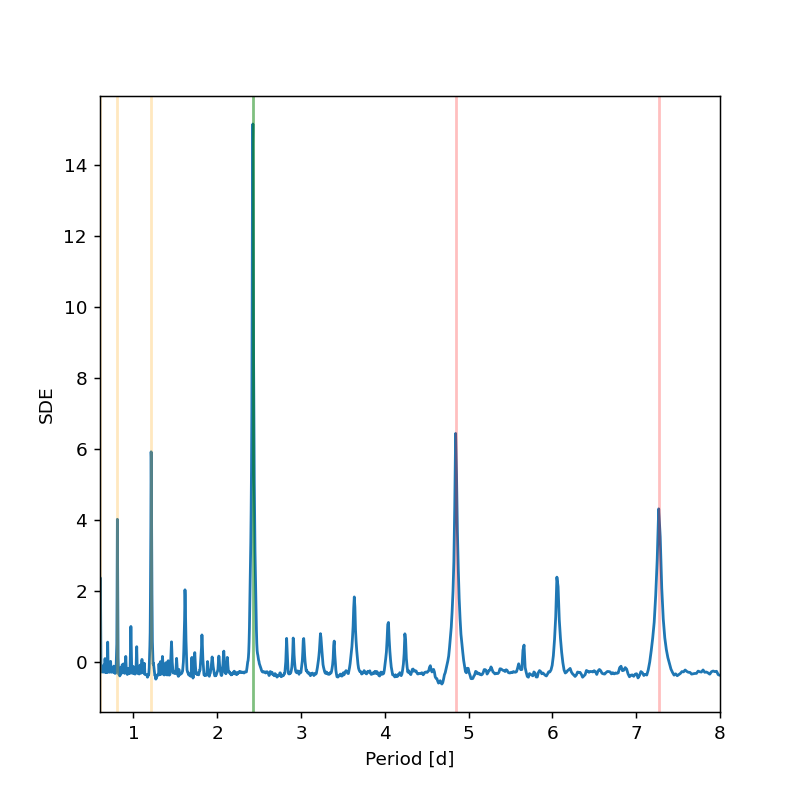
\includegraphics[scale=0.3, angle=0]{../pictures/tess/sde.png}
    \caption{TLS periodgram}
%   \label{fig:Transits}
\end{figure}

\begin{figure}
  \centering
    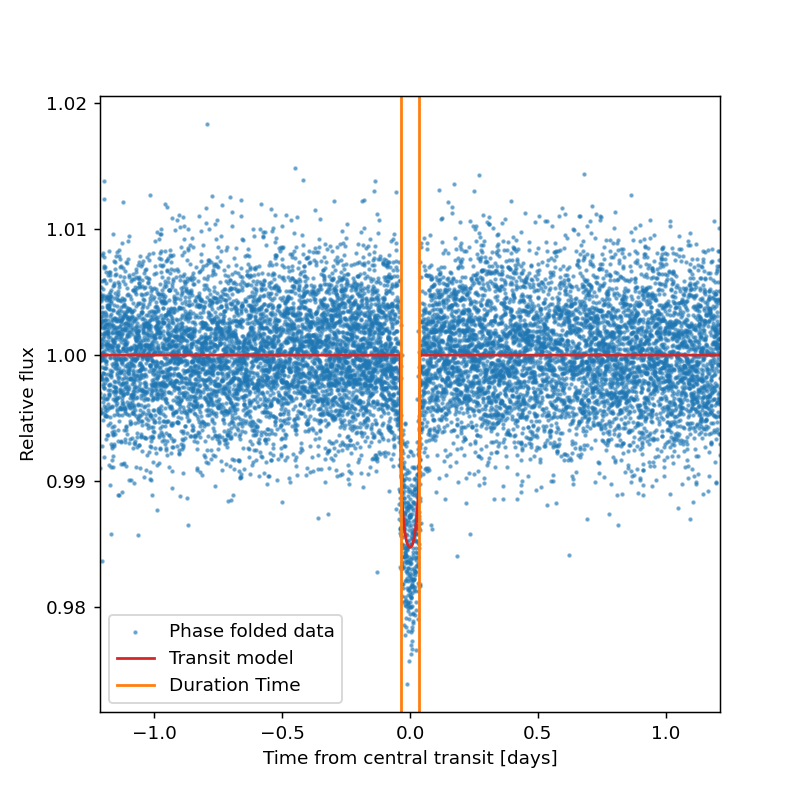
\includegraphics[scale=0.3, angle=0]{../pictures/tess/transit.png}
    \caption{Detrended transits}
 %  \label{fig:Transits}
\end{figure}

At last, we chose to select only the data points that are at a distance which is within twice the value of the transit duration from the center of the transit, 
we saved the output in a data file that will be the basis for the subsequent analysis and we plotted the resulting transit light curve.
\begin{figure}
  \centering
    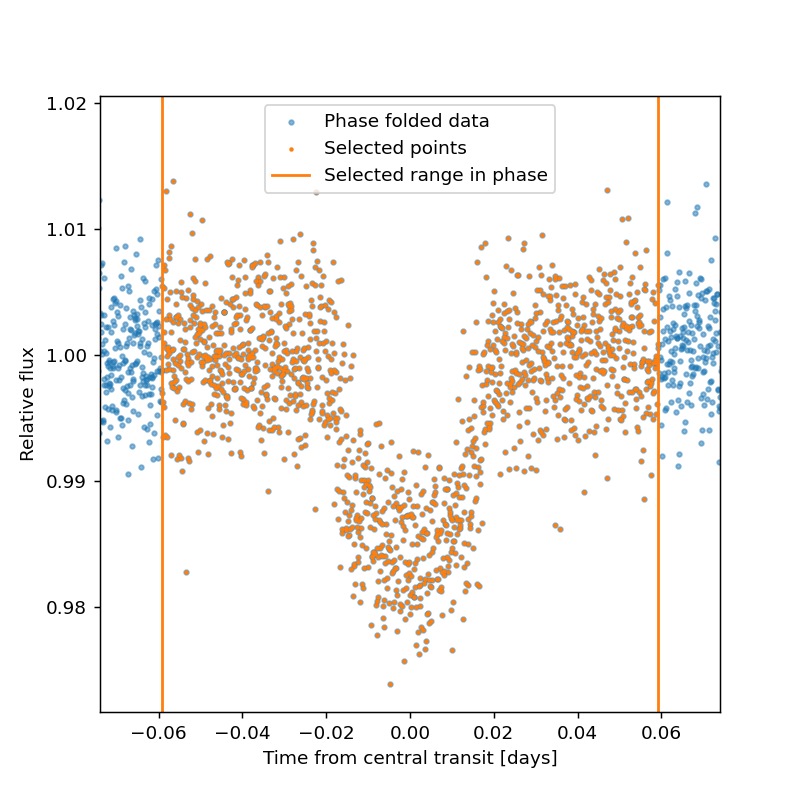
\includegraphics[scale=0.3, angle=0]{../pictures/tess/final.png}
    \caption{Final selection}
 %  \label{fig:Transits}
\end{figure}

\newpage

\section{Light curve fit}

%Conversion from fit parameters to physical parameters
Once obtained the datasets and prepared the configuration files written in YAML language both for TASTE and TESS, we proceeded to fit the transit light curves with a planetary model.

To this aim we performed the analysis using \textit{PyORBIT}\footnote{https://github.com/LucaMalavolta/PyORBIT} (\cite{Malavolta16}, \cite{Malavolta18}), a framework for the characterization of planetary systems that is able to analyse photometry, RVs and ancillary data and model stellar activity and transit time variations.

All the planetary transits were modelled using the Python package \textit{BATMAN} (\cite{Kreidberg}); we used also the differential evolution tool \textit{PyDE}\footnote{https://github.com/hpparvi/PyDE} in combination with the affine-invariant Markov chain Monte Carlo (MCMC) sampler \textit{EMCEE} (\cite{Foreman}) to perform global optimization of the input parameters and an autocorrelation analysis of the chains.

In the chosen models the orbits were assumed to be tidally circularized, and a jitter flag was activated in order to add a jitter parameter in quadrature to the flux errors to compensate their under-estimation.

For the Bayesian analysis of the TESS lightcurve, we assumed a circular orbit, a quadratic law for the limb darkening coefficients, uniform priors for the period, the central time of transit, the impact parameter, the scaled planetary radius, and gaussian priors for the stellar parameters.


For the Bayesian analysis of the TASTE lightcurve, we chose a second order polynomial trend as a model for out of transit flattening, gaussian priors for the period, the limb darkening coefficients, the stellar parameters and uniform priors for all the other parameters.

Since the resulting chains were more than 50 times longer than the autocorrelation function, we are assured that the estimate can be trusted.

The physical parameters obtained from the posterior samples are collected in tables \ref{table:1} and \ref{table:3} in the following sections.

%\ref{table:2} for TESS and Tables for TASTE.
The corner plots of the posterior samples showing the correlation between the parameters are reported in Fig. \ref{fig: cptess}, \ref{fig: cptaste} and \ref{fig: ptrend} .

Along the diagonal there are histograms of the estimated 1D posterior probability distribution for each parameter. 

The histograms show that the recovered parameters are both accurate (close to injected value) and precise (narrow posterior distribution). 

The off-diagonal plots are the 2D histograms of the estimated joint posterior probability distribution of each pair of parameters, which show the correlation between pairs of parameters.

The normalized stellar fluxes, fitted with the model of the exoplanetary transit, along with the residuals are reported in Fig. \ref{fig: lc1} and \ref{fig: lc2} .

\subsection{TESS}




 \begin{table}[h!]
 \centering
    \begin{tabular}{cccc}
    \hline
     Parameter& Value & $\sigma_{-}$ & $\sigma_{+}$\\
    \hline
    P ($d_{BJD}$)   &  2.423846   &  0.000168 &     0.000167 \\
    $T_{c} (d_{BJD})$ &  2458386.578204 & 0.000720  & 0.000721  \\ 
    b & 0.526068  & 0.052957    & 0.047805  \\
    $R_{P }/ R_{\star}$&  0.116950 & 0.002680   &  0.002595\\
    $\rho (\rho_{\odot})$ & 1.209717 & 0.088844  &  0.090123\\
    $c1_{ld}$ & 0.509840    & 0.282570  & 0.257019\\
    $c2_{ld}$ &0.167904 & 0.392996 & 0.396461\\
    jitter & 0.000241 &0.000141 &0.000219 \\
    \hline
    \end{tabular} 
  \caption{Physical parameters obtained from TESS analysis}
 \label{table:1}
 \end{table}



\begin{figure}
  \centering
    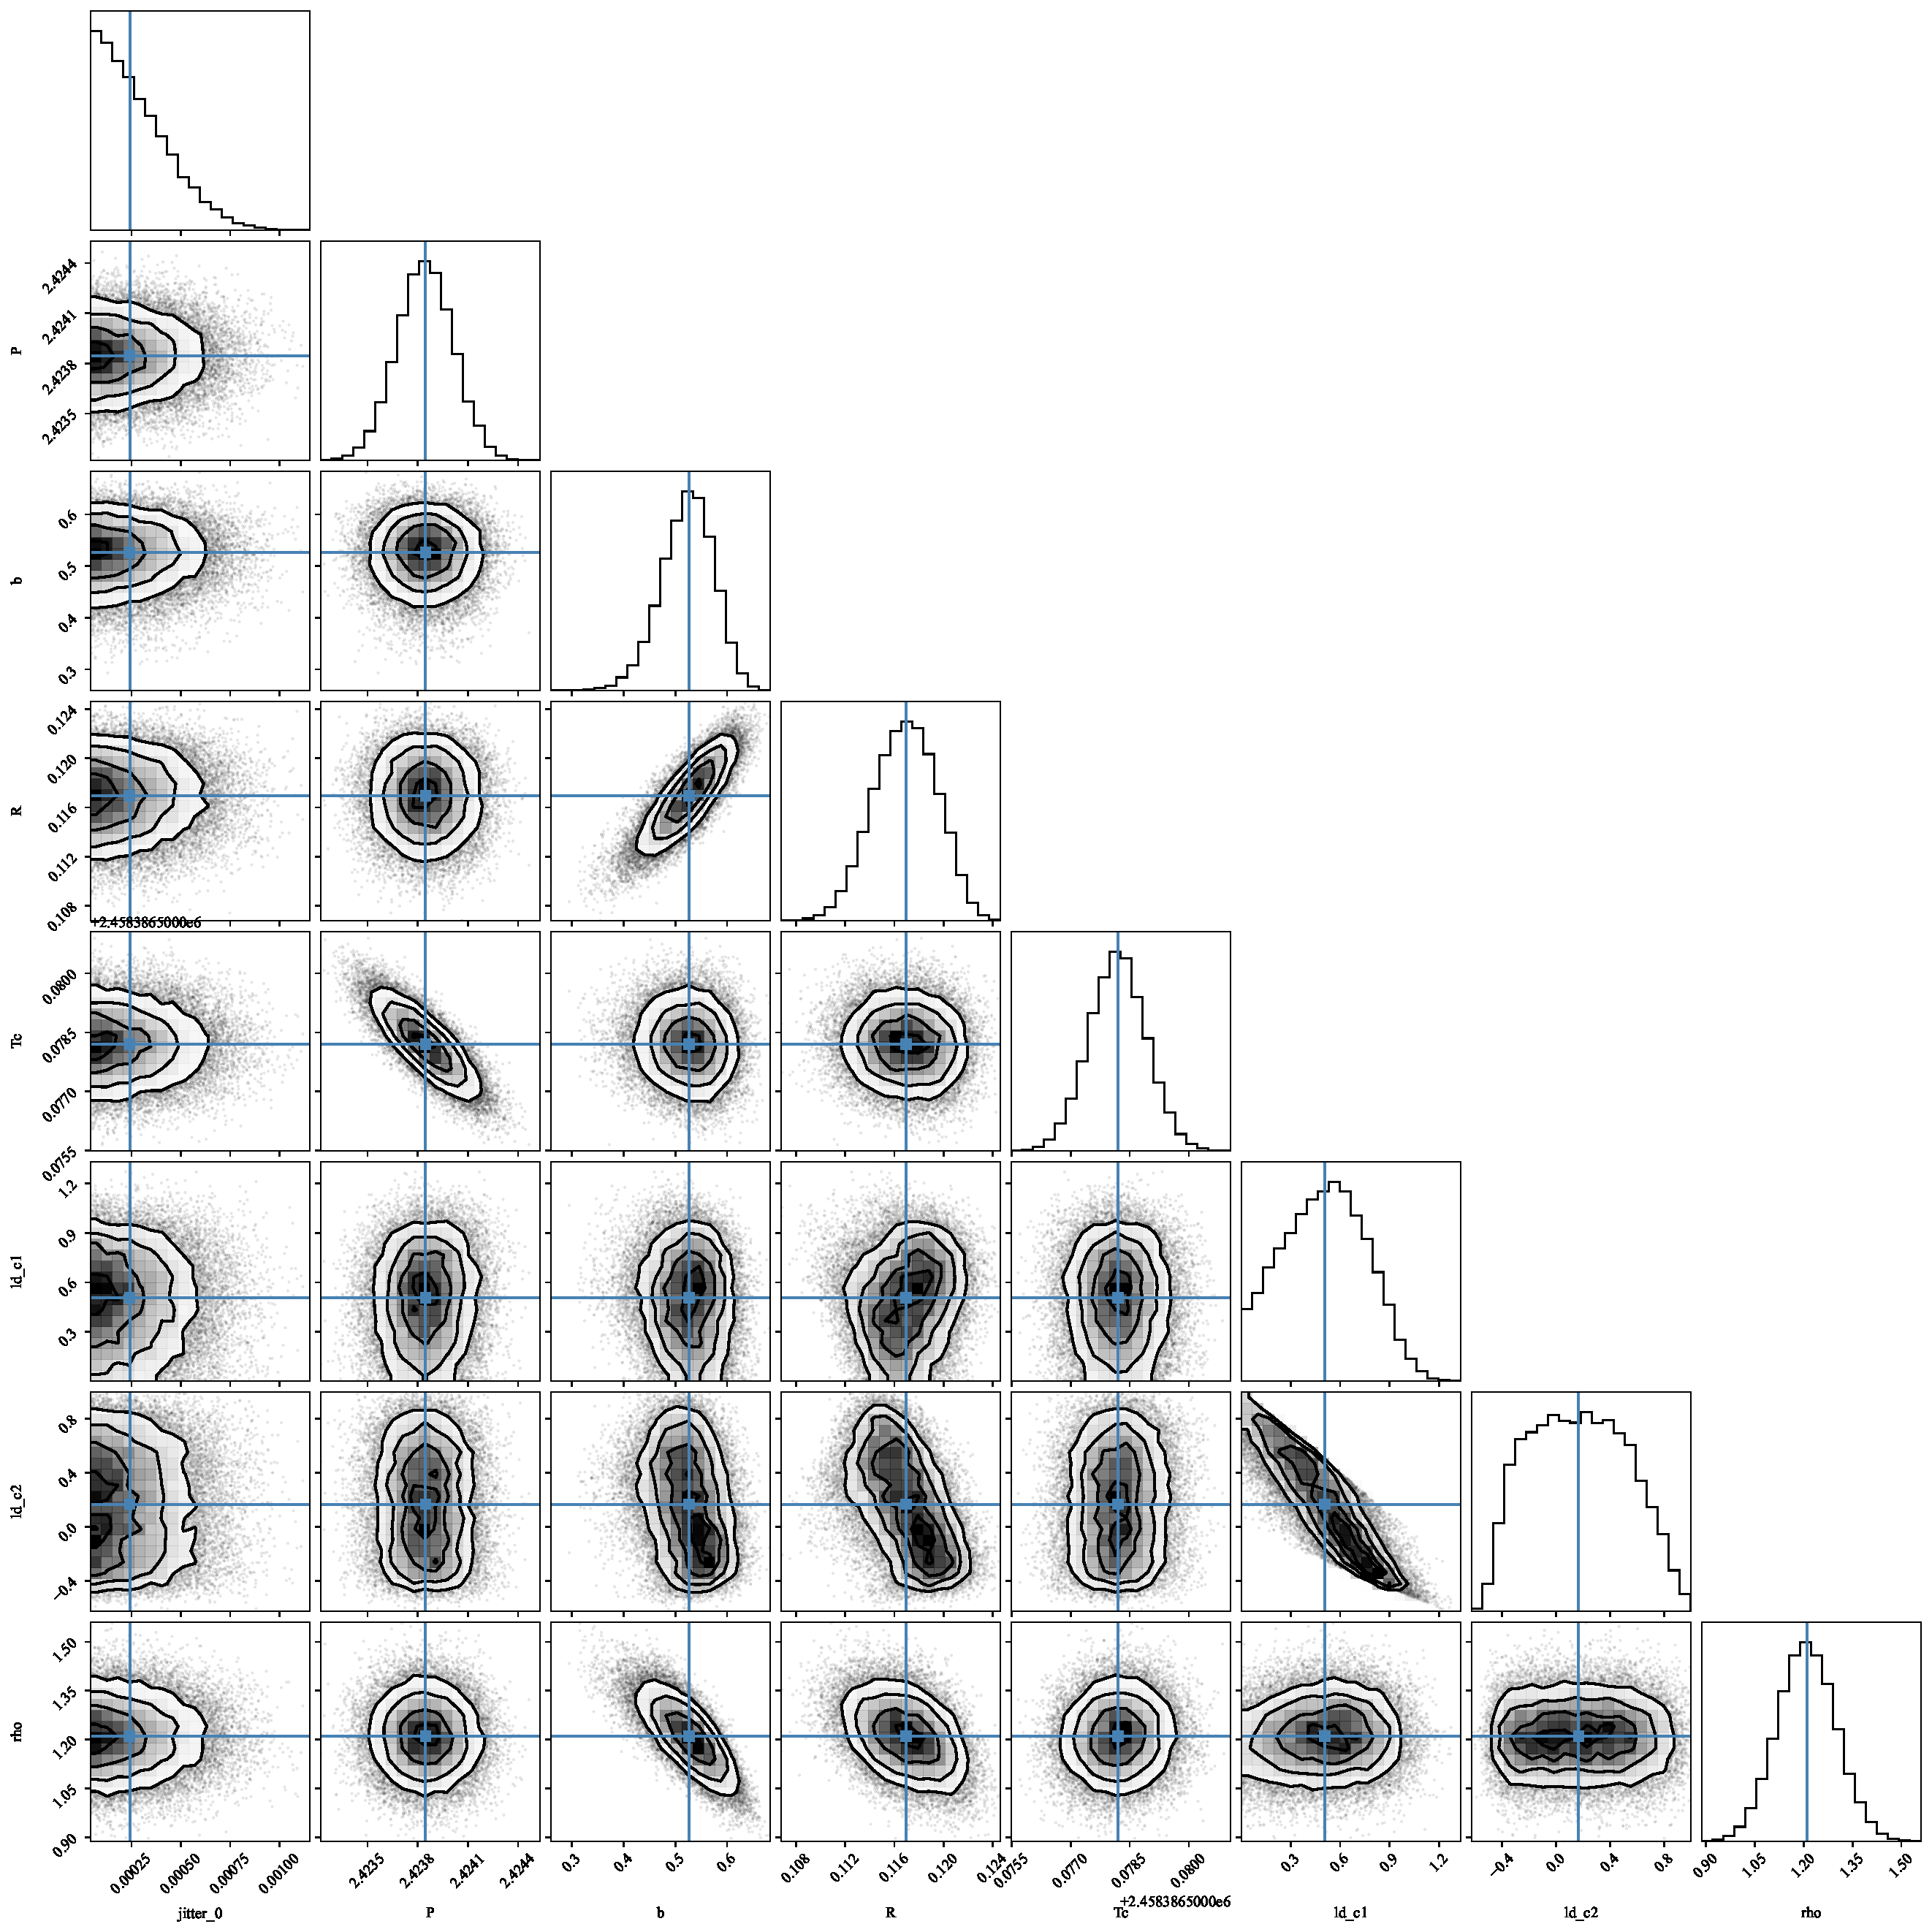
\includegraphics[scale=0.2, angle=0]{../pictures/tess/acf_tess.pdf}
     \caption{Full variables TESS corner plot}
    \label{fig: cptess}
\end{figure}


\begin{figure}
  \centering
    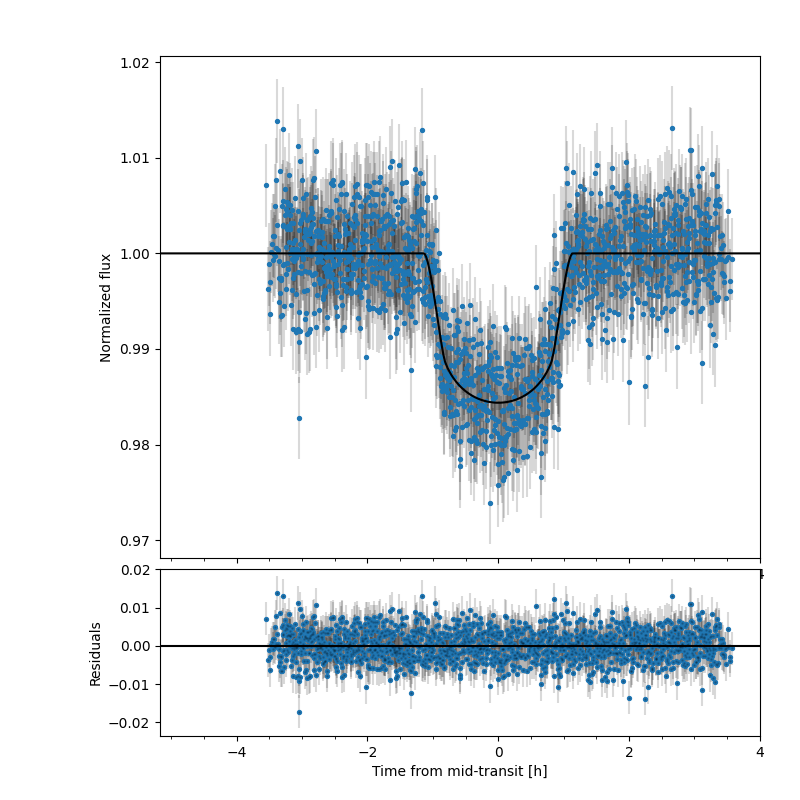
\includegraphics[scale=0.3, angle=0]{../pictures/tess/lctess.png}
    \caption{TESS lightcurve}
   \label{fig: lc1}
\end{figure}

\newpage
\subsection{TASTE}


 \begin{table}[h!]
 \centering
    \begin{tabular}{cccc}
    \hline
     Parameter& Value & $\sigma_{-}$ & $\sigma_{+}$\\
    \hline
    P ($d_{BJD}$)   &  2.468733    &  0.158915  &  0.131093 \\
    $T_{c} (d_{BJD})$ &  2459174.317823 & 0.000566  &  0.000554  \\ 
    b &  0.585133  & 0.051438    &  0.042263  \\
    $R_{P }/ R_{\star}$ & 0.129397 & 0.003821 &  0.003747 \\
    $\rho (\rho_{\odot})$ & 1.156424 &0.088183   &   0.090487 \\
    $c1_{ld}$ &  0.345531     & 0.090242  &  0.091553 \\
    $c2_{ld}$ &0.230632 & 0.098916 &0.099288\\
    jitter & 0.003067  &0.000359  &0.000341\\
    $p_{0}$ & 1.053690  & 0.001014&  0.001026\\
    $p_{1}$ &0.001706 &0.004975  & 0.004923\\
    $p_{2}$ &0.553433  &0.218298  & 0.211560\\ 
    \hline
    \end{tabular} 
   \caption{Physical parameters obtained from TASTE analysis}
 \label{table:3}
 \end{table}


\begin{figure}
  \centering
    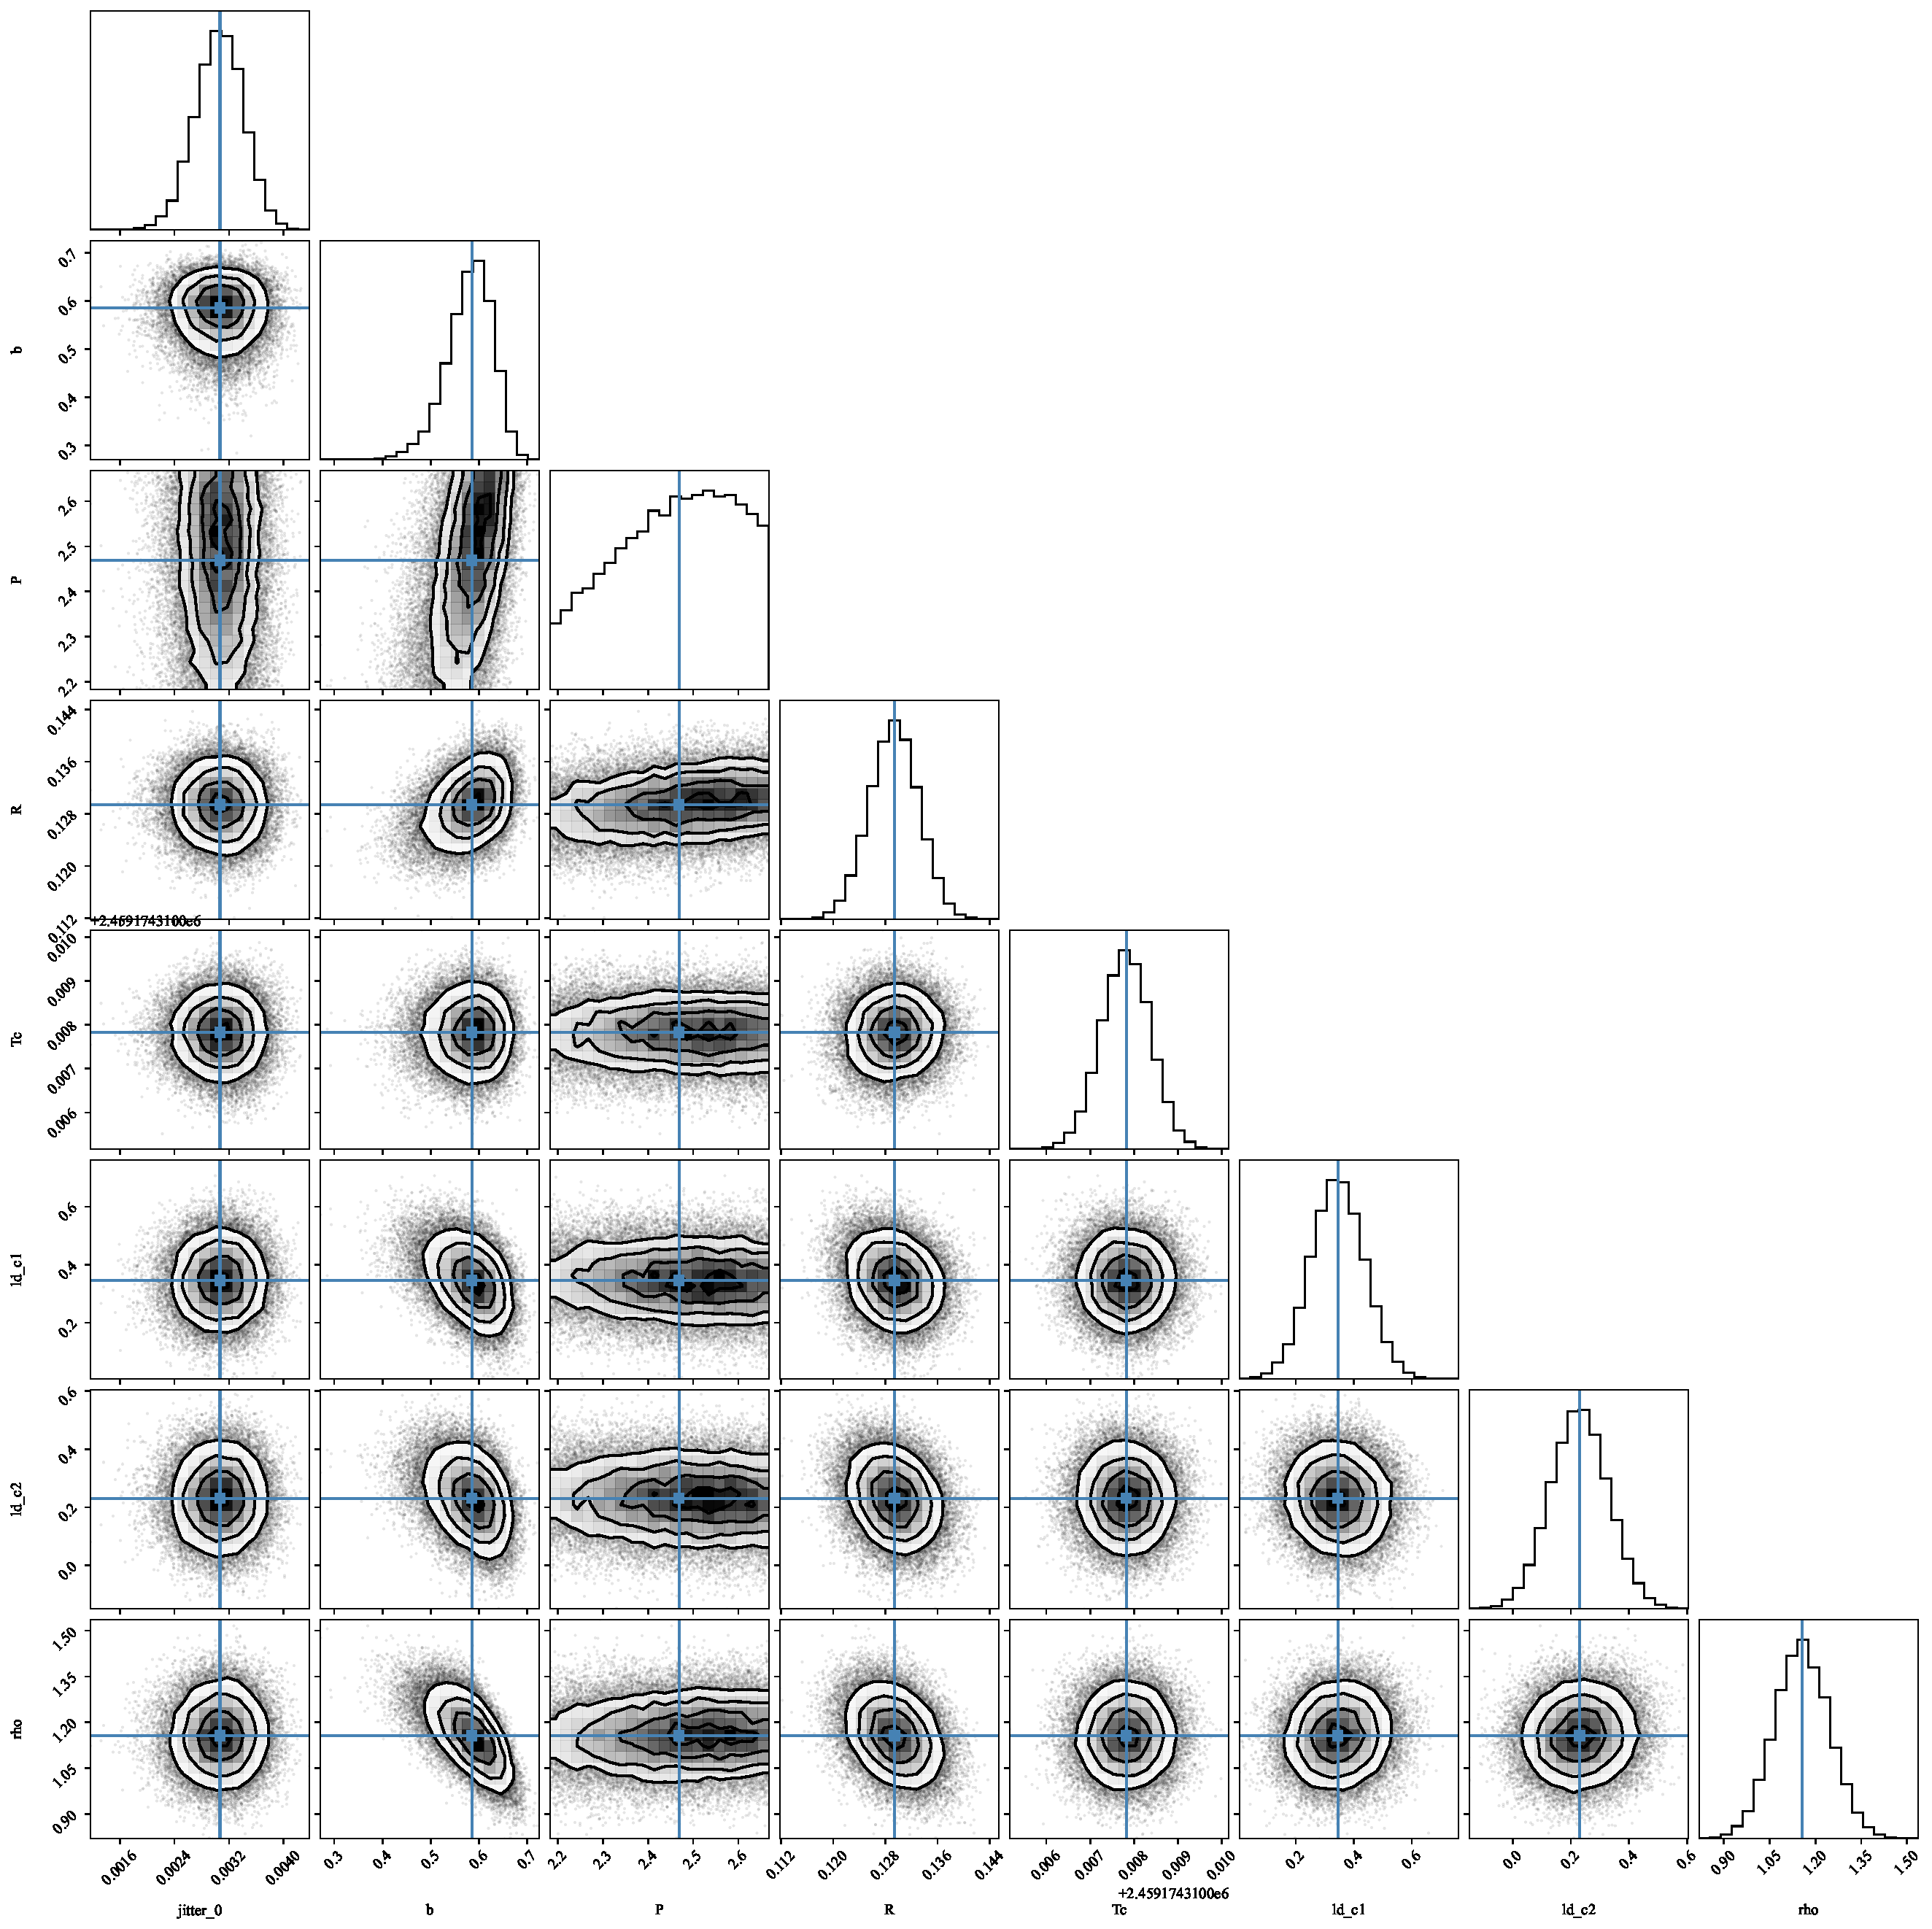
\includegraphics[scale=0.2, angle=0]{../pictures/taste/acf_taste.pdf}
    \caption{Correlation between all the TASTE variables}
   \label{fig: cptaste}
\end{figure}


\begin{figure}
  \centering
    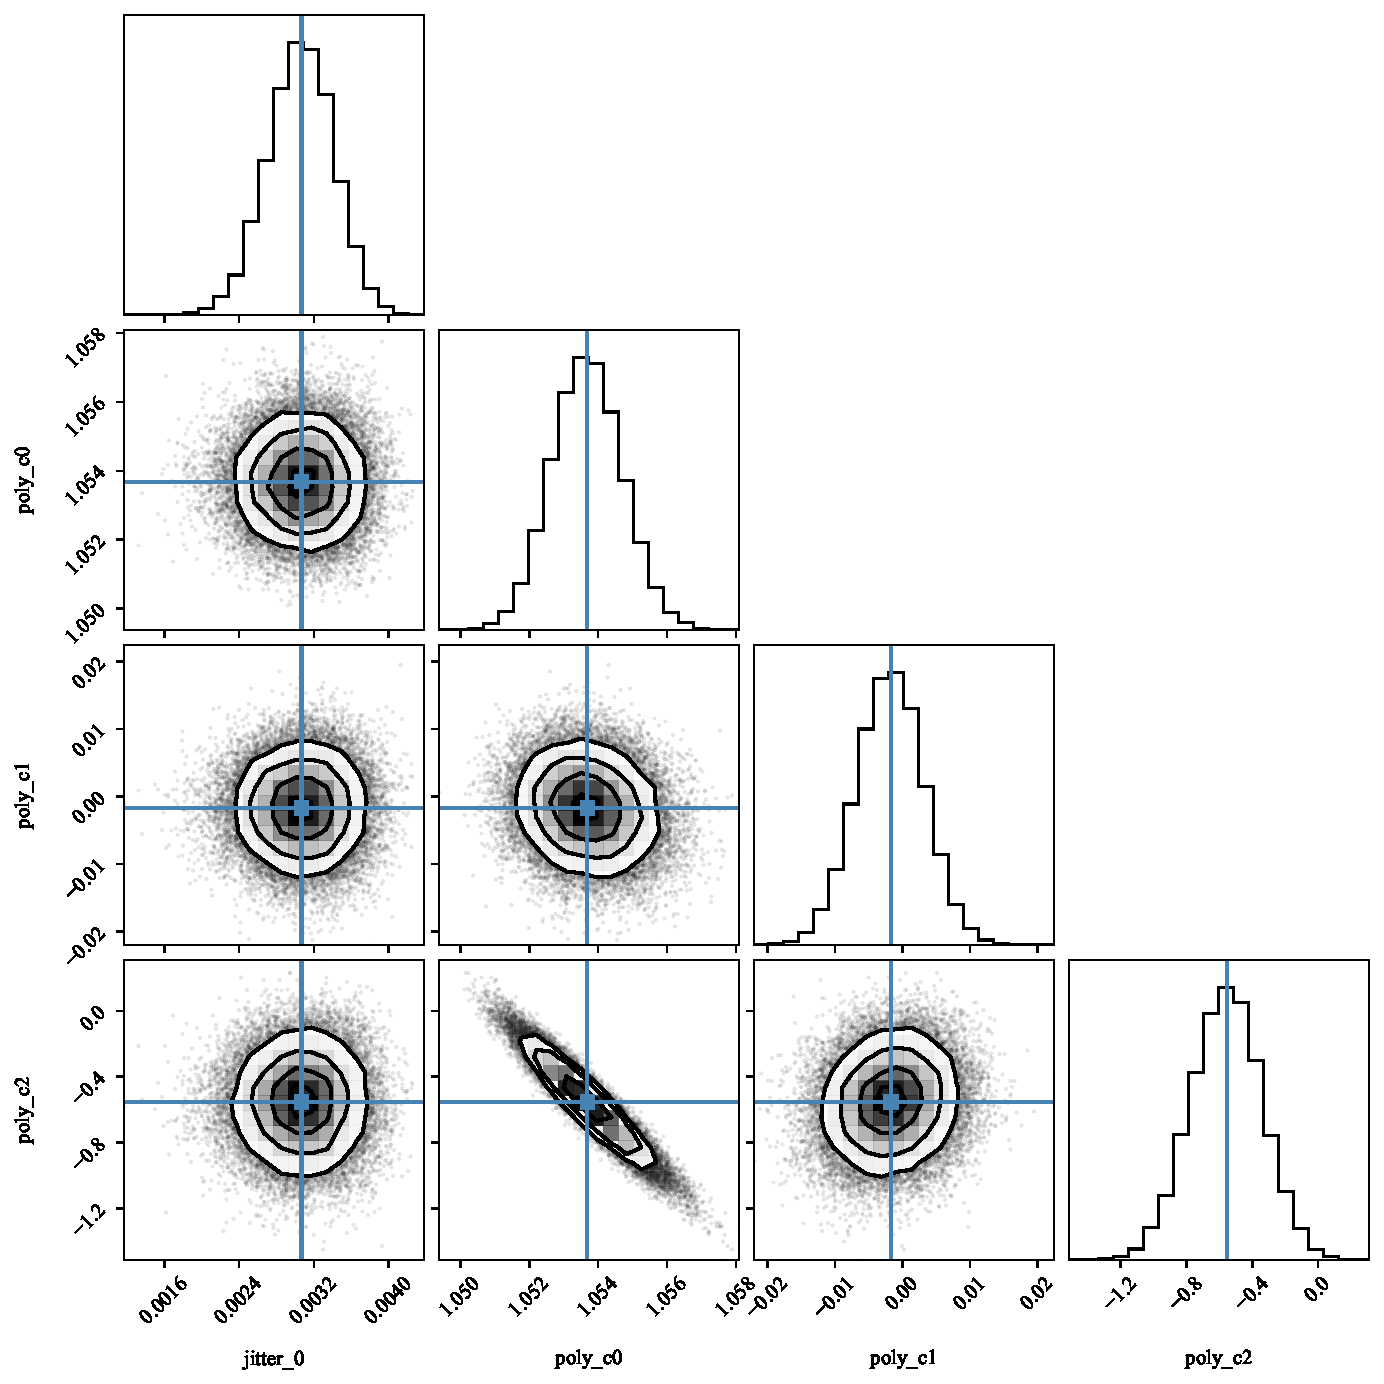
\includegraphics[scale=0.3, angle=0]{../pictures/taste/poly.pdf}
    \caption{Polynomial trend corner plot}
   \label{fig: ptrend}
\end{figure}


\begin{figure}
  \centering
    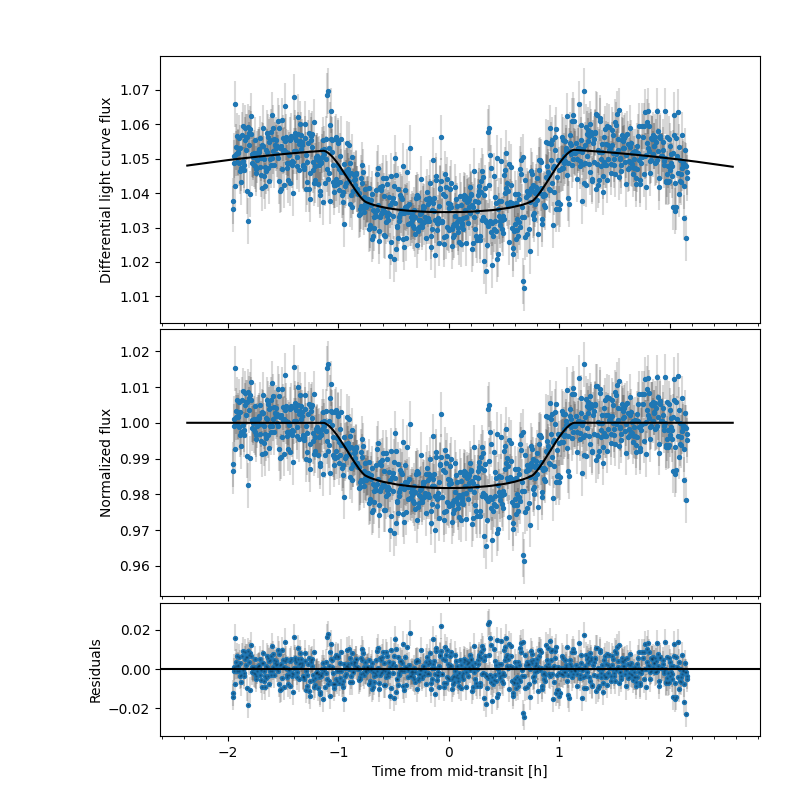
\includegraphics[scale=0.3, angle=0]{../pictures/taste/lctaste.png}
    \caption{TASTE lightcurve}
   \label{fig: lc2}
\end{figure}




\subsection{Comparison}

As a further check on the output values of our analysis, we apply 
the (OC) method in order to compare the observed (O)
central transit time (from TASTE observations) to the expected calculated (C) value (TESS results) .

We obtain a O-C value of -0.010331 which indicates the accuracy of our analysis.

\begin{figure}
  \centering
    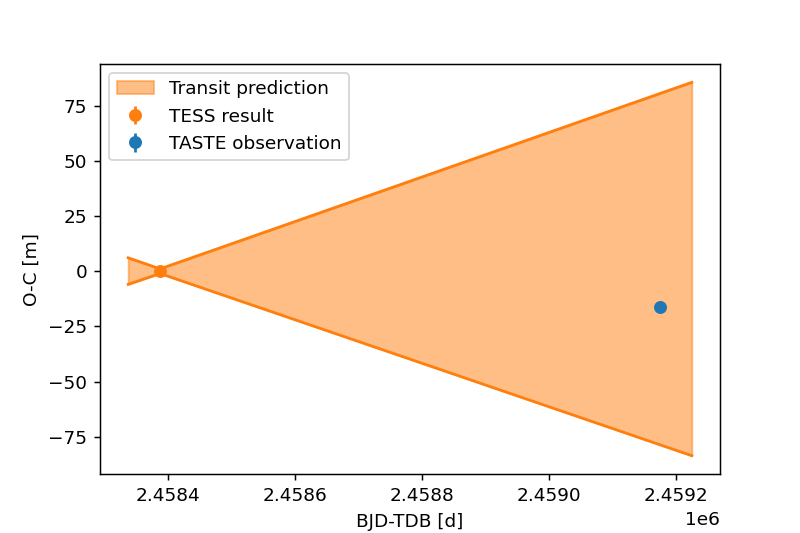
\includegraphics[scale=0.4, angle=0]{../pictures/comparison/oc.png}
    \caption{O-C plot}
 %  \label{fig: ocplot}
\end{figure}


\newpage

\section{Radial velocity analysis}
Knowing the RV semi-amplitude $K_*$ and the mass $M_*$ of the star,
the planetary mass $M_p$ is obtained by inverting the following equation. 
\begin{equation}
    K_* = \frac{1}{\sqrt{1-e^2}}\frac{M_p \sin{i}}{(M_*+M_p)^{2/3}}\left(\frac{P}{2\pi G}\right)^{-1/3}
\end{equation}
where $M_p\sin{i}$ represents a \textit{minimum mass} estimate. $i$ can be 
measured for a transiting planet, thus yielding $M_p$.
Velocity was observed by hashafasha. Only one radial velocity time series
is available at NASA Exoplanet Archive \footnote{https://exoplanetarchive.ipac.caltech.edu/}, 
involving 17 points and based on optical band spectral measurements 
(\cite{Anderson}). CORALIE spectrograph mounted on the 1.2-m
Euler-Swiss telescope was used in 2010 to gather the 17 spectra that lead
to this RV dataset. We made sure the time range of this set did not overlap 
with the time range of the transits: any stellar spectra taken while the planet is 
transiting is missing a contribution and can be no longer considered as a RV 
datapoint.
We ran PyORBIT again to fit the RV curve with a proper model. Radial velocity input
file can be equipped with an extra "0" column, in order to enable the code to compute
any RV offset due to the peculiar velocity of the star.
Two models were exploited for the analysis: \textit{radial velocities} and 
\textit{harmonics}.
\begin{table}[h!]
    \centering
       \begin{tabular}{cccc}
       \hline
        Par& Value & $\sigma_{-}$ & $\sigma_{+}$\\
       \hline
		$jitter$ &            8.186931  &        -5.674228  &       8.840726 \\
		$offset$ &         -4044.009310 &        -6.587574 &        7.142502 \\
	    $P$   &2.423806        & -0.000022   &      0.000021   \\
	    $T_c$  &2458386.578204  & -0.000728   &      0.000726  \\
	    $K$   &137.437324      & -10.397997  &      10.170602\\
       \hline
       \end{tabular} 
     \caption{Physical parameters obtained for \textit{radial velocities} model.}
\end{table}

\begin{figure}
	\centering
	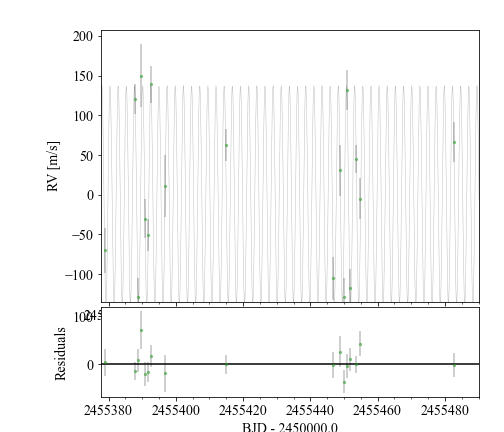
\includegraphics[scale=0.4, angle=0]{../pictures/RV/RV_unfolded.png}
	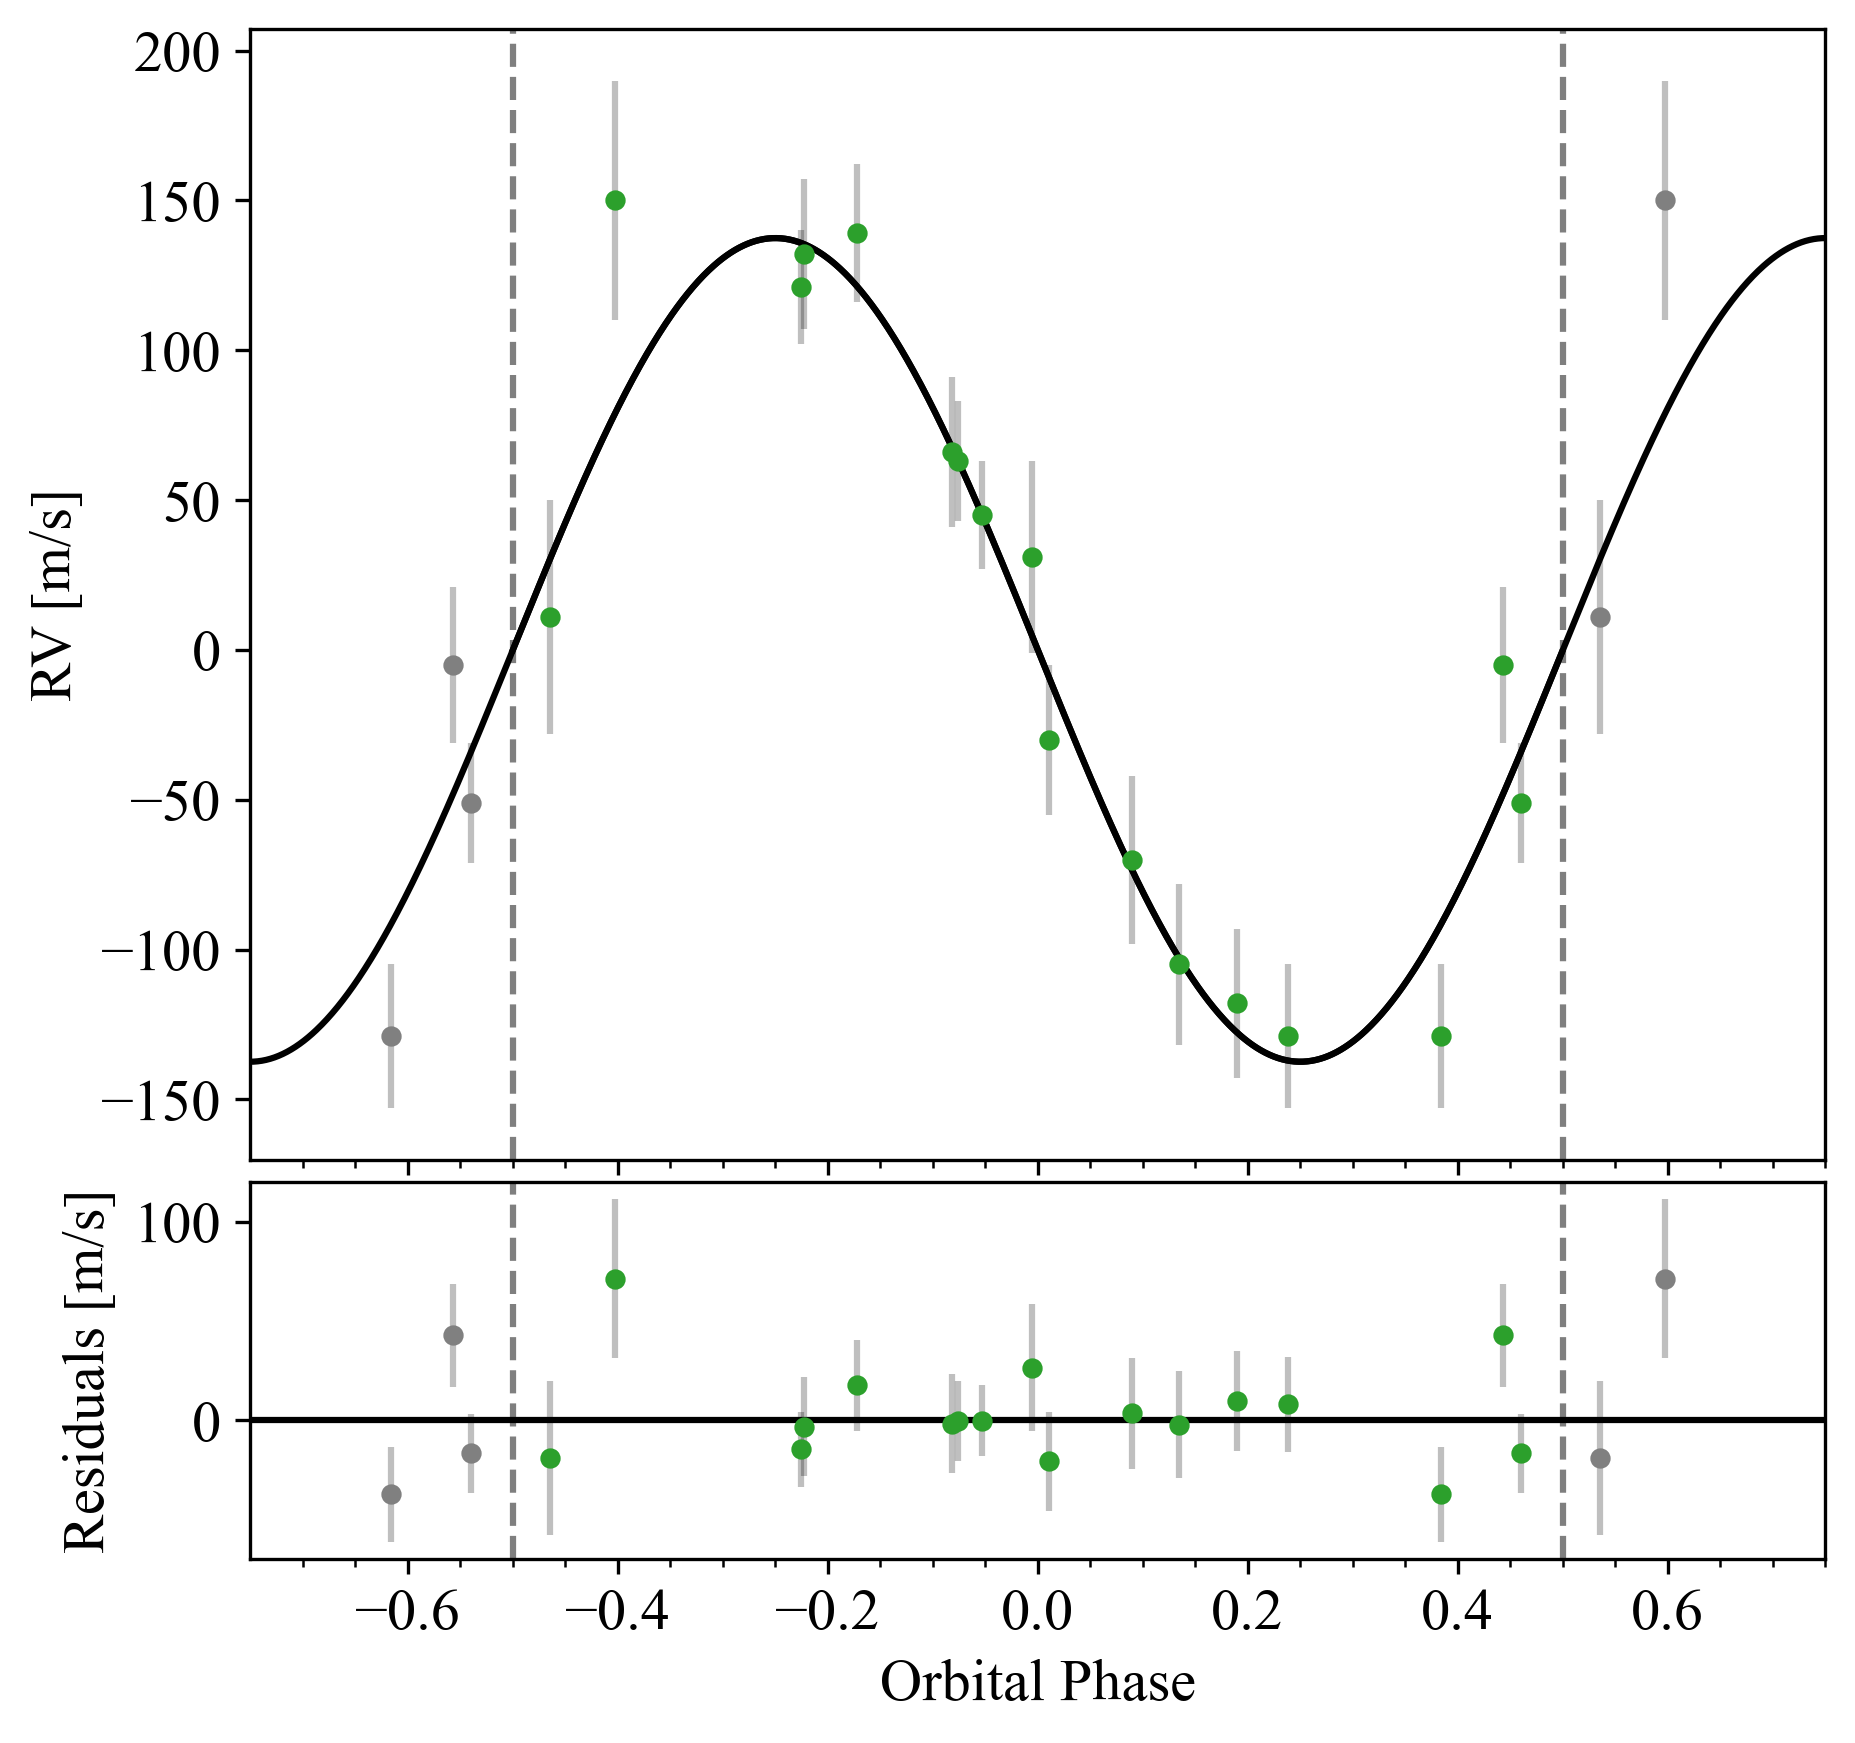
\includegraphics[scale=0.4, angle=0]{../pictures/RV/RV.png}
	\caption{Radial velocities fitting, unfolded and folded model.}
	\label{fig:RV1}
\end{figure}

As for the second model:
\begin{table}[h!]
	\centering
	\begin{tabular}{cccc}
		\hline
		Par& Value & $\sigma_{-}$ & $\sigma_{+}$\\
		\hline
		$jitter$ &            8.412502 &        -5.733187  &       9.012852 \\
		$offset$ &         -4043.655266 &        -7.025075 &        7.166508 \\
		$P$   &2.423806       & -0.000029    &      0.000028   \\
		$T_c$  &2458386.578202  & -0.000708   &      0.000741  \\
		$K$   &137.052049      & -14.095483  &      13.019732\\
		\hline
		Stellar par& Value & $\sigma_{-}$ & $\sigma_{+}$\\
		\hline
		$P$ &            2.423850 &        -0.000166   &       0.000167 \\
		$phase$ &         7.003042  &        -2.175383 &        2.084340  \\
		\hline
	\end{tabular} 
	\caption{Physical parameters obtained for \textit{harmonics} model.}
\end{table}

\begin{figure}
	\centering
	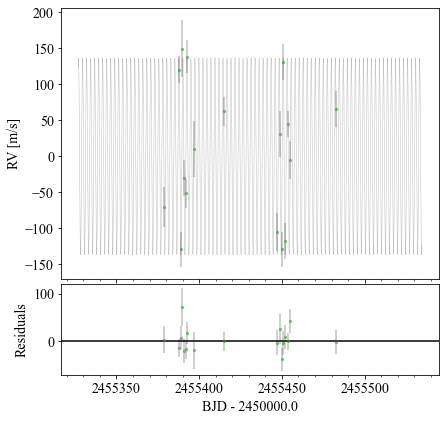
\includegraphics[scale=0.4, angle=0]{../pictures/RV/RV2_unfolded.png}
	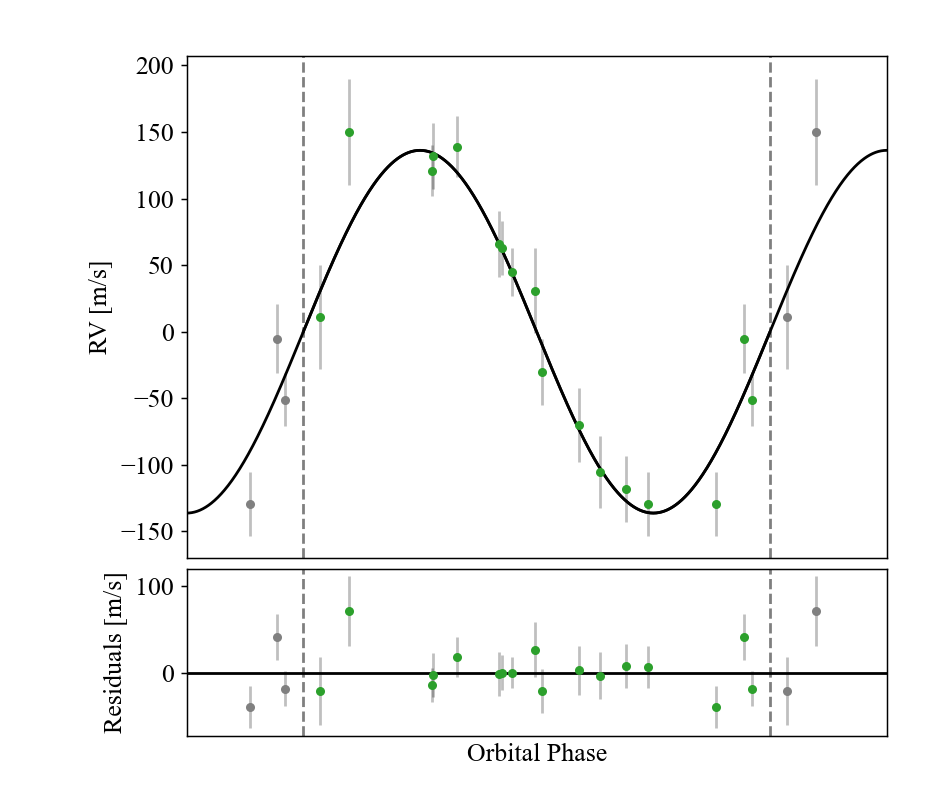
\includegraphics[scale=0.4, angle=0]{../pictures/RV/RV2.png}
	\caption{Radial velocities fitting, unfolded and folded model.}
	\label{fig:RV2}
\end{figure}

\newpage

\section{Conclusions}















\appendix
\section{Limb darkening analysis}
\label{sect:app_A}

\subsection{Claret 2017}
We can represent data tables in \cite{claret2017} as 2D histograms, 
after proper unfolding of the data tables attached to the paper. To do that, 
we first fix metallicity, then gravity and see how the corresponding LD 
coefficients $c_1$ and $c_2$ depend on all three atmospheric parameters. 
\begin{figure}[H]
    \centering  
    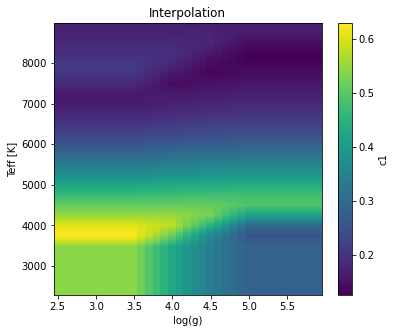
\includegraphics[scale=0.25, angle=0]{../pictures/Claret2017/2017_c1_fixedmet}
    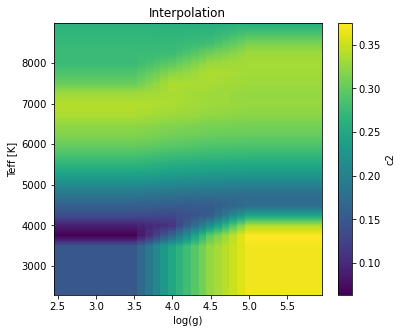
\includegraphics[scale=0.25, angle=0]{../pictures/Claret2017/2017_c2_fixedmet}

    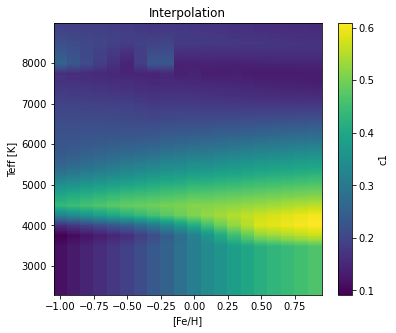
\includegraphics[scale=0.25, angle=0]{../pictures/Claret2017/2017_c1_fixedg}
    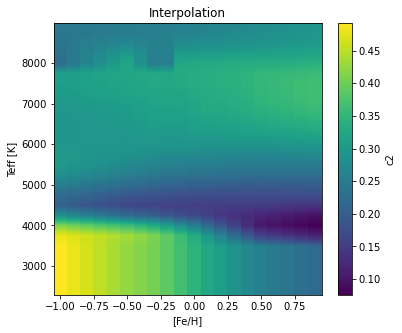
\includegraphics[scale=0.25, angle=0]{../pictures/Claret2017/2017_c2_fixedg}
    \caption{LD coefficient with fixed metallicty, fixed gravity}
\end{figure}
Furthermore, it's very interesting to check the strength of the dependance 
on each atmospheric parameters. Turns out LD coefficients are essentially a 
function of temperature, and minor dependences on gravity and metallicity 
can be barely appreciated.
\begin{figure}[H]
    \centering  
    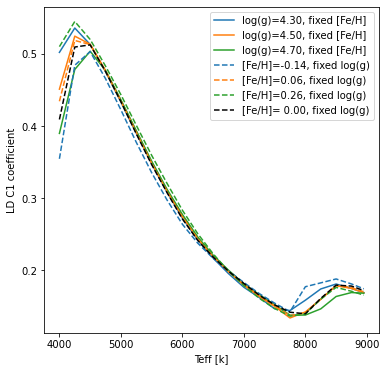
\includegraphics[scale=0.25, angle=0]{../pictures/Claret2017/2017_c1}
    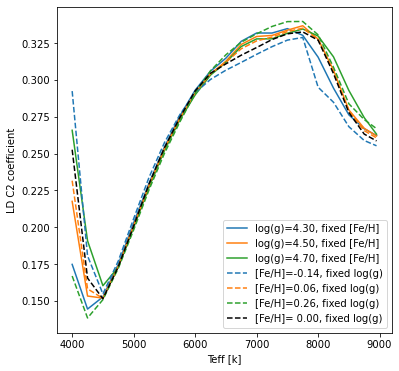
\includegraphics[scale=0.25, angle=0]{../pictures/Claret2017/2017_c2}
    \caption{LD coefficient as a function of atmospheric parameters}
\end{figure}
A relevant dependance on gravity and metallicity can only be noticed at 
high temperatures, where we should carefully select the proper curve. But 
in the range we're interested in ($\approx 5400 K$) the curve is 
degenerate and the choice of these parameters is secondary.

We perform a Montecarlo simulation, generating 1000 random atmospheric 
parameters around the actual ones. Even in this case we see that the 
distribution of the fixed-metallicity estimates is almost overlapping 
with the fixed-gravity one, thus confirming $c_1$ and $c_2$ not very 
sensitive on metallicity and gravity.
\begin{figure}[H]
    \centering  
    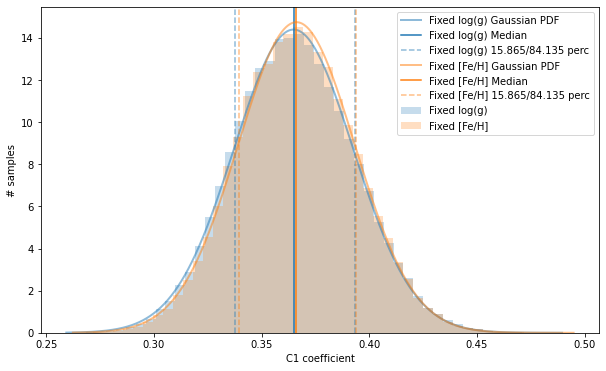
\includegraphics[scale=0.35, angle=0]{../pictures/Claret2017/2017_c1_comp}
    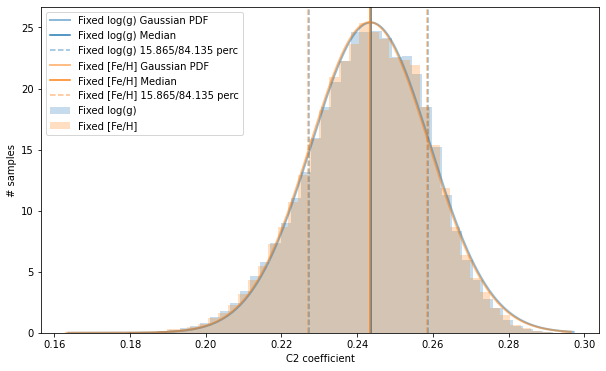
\includegraphics[scale=0.35, angle=0]{../pictures/Claret2017/2017_c2_comp}
    \caption{Montecarlo simulation for $c_1$ and $c_2$, for fixed metallicity 
    and for fixed gravity}
\end{figure}
The two estimates are well compatible, thus authorizing a weighted average: 
$c_1 = 0.366 \pm 0.019$ and $c_2 = 0.243 \pm 0.011$.

Another way to deal with the same table is by selecting from the set two values
of metallicity or gravity, an upper and lower limit, instead of just one reference 
value. This way we build two matrices and 
interpolate between the two to get to the desired result. The rest of the procedure is 
the same as just explained, leading to other estimate of the LD coefficients.
\begin{figure}[H]
    \centering  
    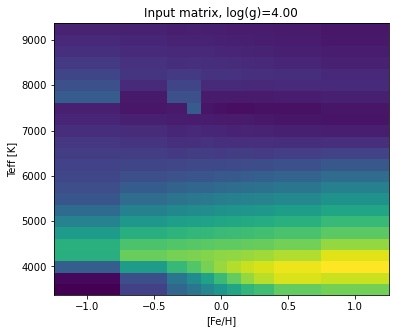
\includegraphics[scale=0.35, angle=0]{../pictures/Claret2017/double_logg4}
    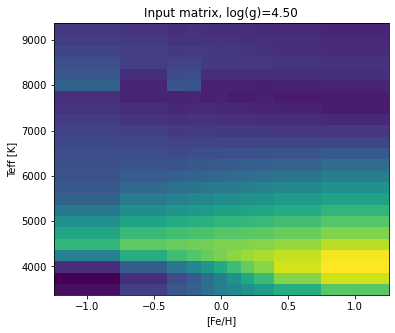
\includegraphics[scale=0.35, angle=0]{../pictures/Claret2017/double_logg45}
    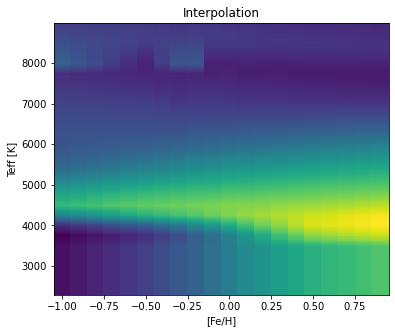
\includegraphics[scale=0.35, angle=0]{../pictures/Claret2017/double_logg_interp}
    \caption{Matrices obtained by fixing gravity to $\log{g}=4.0$ to $4.5$, plus the interpolated matrix}
\end{figure}
\begin{figure}[H]
    \centering  
    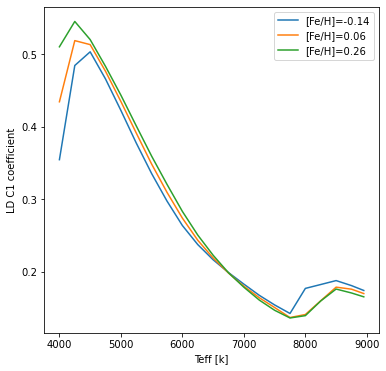
\includegraphics[scale=0.35, angle=0]{../pictures/Claret2017/double_c1}
    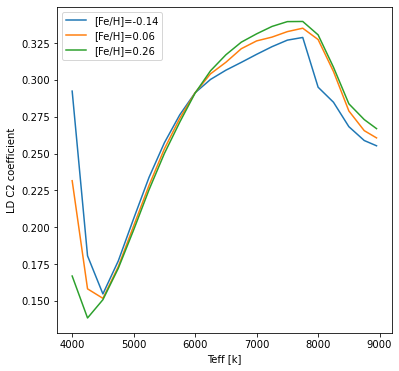
\includegraphics[scale=0.35, angle=0]{../pictures/Claret2017/double_c2}
    \caption{LD coefficients trend in the $T_{eff}-[Fe/H]$ plane}
\end{figure}
This can be done in the same exact way by fixing metallicity instead.

\subsection{Claret 2018}
A successive paper provided a new method to model the LD coefficients dependency 
on atmospheric parameters. We'd like to check if this leads to different results 
with respect to the 2017 paper. Unfolding the table requires the same procedure 
we've already described. Just note that in both cases we fix metallicity, and for 
the 2018 table metallicity must be fixed to 0, since the method is conceived for
zero-metallicity stars.
\begin{figure}[H]
    \centering  
    \includegraphics[scale=0.35, angle=0]{../pictures/ClaretvClaret/2017.png}
    \includegraphics[scale=0.35, angle=0]{../pictures/ClaretvClaret/2018.png}
    \caption{Final, interpolated matrices for the two methods (2017 left, 2018 right)}
\end{figure}
And finally we can display the dependency of the LD coefficients for the 
two-parameters game.
\begin{figure}[H]
    \centering  
    \includegraphics[scale=0.35, angle=0]{../pictures/ClaretvClaret/c1.png}
    \includegraphics[scale=0.35, angle=0]{../pictures/ClaretvClaret/c2.png}
    \includegraphics[scale=0.35, angle=0]{../pictures/ClaretvClaret/c1_comp.png}
    \includegraphics[scale=0.35, angle=0]{../pictures/ClaretvClaret/c2_comp.png}
    \caption{$c_1$ and $c_2$ trend, and comparison between the final results}
\end{figure}
See how there is an actual difference between the adopted methods, that lead 
in fact to slightly different results for the LD coefficients. The good news is, 
they're largely compatible: see how each value is within a few errorbars away 
from the other.

\subsection{Claret 2011}
We use another table from an older paper by the same author, where even 
filters have a role. By looking at the header of our dataset, we find the 
right filter to be $r^{*}$ (SDSS). Remember that transits look differently 
when observed through different filters, and also that boxier transits make 
ingress/egress time determination easier. The unfolding technique is always 
the same.
This time, we account for stellar models (ATLAS/PHOENIX) and interpolation 
technique (least squares/flux conservation), for a grand total of 4 
combinations. These are the very final results.
\begin{figure}[H]
    \centering  
    \includegraphics[scale=0.35, angle=0]{../pictures/Claret2011/c1.png}
    \includegraphics[scale=0.35, angle=0]{../pictures/Claret2011/c2.png}
    \includegraphics[scale=0.35, angle=0]{../pictures/Claret2011/c1_comp.png}
    \includegraphics[scale=0.35, angle=0]{../pictures/Claret2011/c2_comp.png}
    \caption{$c_1$ and $c_2$ trend, and comparison between the final results}
\end{figure}
Again, all results are fully compatible.

\section{Time correction}
When dealing with \textit{sentinel.dat} output, we need to properly convert the 
time series, contained in columns two of the datatable. To do that, first we
convert from minutes to days, then add the zero-point in Julian Date format, and 
finally also add half exposure time (after proper conversion in days).

Moreover, we can make use of the \textit{Time} method to keep count of the time 
taken by the light to travel from the source position to the location of the 
observatory (Cima Ekar, Asiago). Since the Earth is in motion, light time 
travel is variable and follows a sinusoidal behaviour.
\begin{figure}[H]
    \centering  
    \includegraphics[scale=0.55, angle=0]{../pictures/time_corr.png}
\end{figure}

\nocite{*}
\printbibliography

\end{document}